\documentclass[11pt]{article}

% Shared notes settings for Applied Machine Learning lectures (UPES).
% Keep this file free of \documentclass to allow reuse via \input.

\usepackage[utf8]{inputenc}
\usepackage[T1]{fontenc}
\usepackage{lmodern}          % scalable T1 fonts; without this pdflatex falls back
\input{glyphtounicode}        % to bitmapped EC Type 3 and the PDFs are neither
\pdfgentounicode=1            % searchable nor screen-reader friendly
\usepackage[a4paper,margin=1in]{geometry}
\usepackage{hyperref}
\usepackage{xurl}
\usepackage{booktabs}
\usepackage{amsmath}
\usepackage{amssymb}
\usepackage{listings}
\usepackage{xcolor}
\usepackage{enumitem}
\usepackage{parskip}

% Code listings (Python-oriented for this subject).
\lstset{
  language=Python,
  basicstyle=\ttfamily\small,
  keywordstyle=\color{blue},
  commentstyle=\color{gray},
  stringstyle=\color{teal},
  showstringspaces=false,
  columns=fullflexible,
  frame=single,
  framerule=0.2pt,
  breaklines=true
}

\setlist[itemize]{topsep=0.3em,itemsep=0.2em}
\setlist[enumerate]{topsep=0.3em,itemsep=0.2em}

% Simple per-section source line.
\newcommand{\notesources}[1]{\par\noindent{\small\color{gray}\textit{Sources:} \sloppy #1\par}}

% Unit-wise source strings for this subject (used by slides + notes).
% Path is relative to the lecture `latex/` folder (the compilation CWD).
\IfFileExists{../../../_shared/aml-sources.tex}{%
  % Source strings for Applied Machine Learning (CSAI2017P) — used by slides + notes.
% Prescribed texts and reference books are taken from the course syllabus.
% Support texts are the author-hosted open-access editions:
%   statlearning.com            (ISL with Python)
%   probml.github.io/pml-book   (Murphy, Probabilistic Machine Learning)
%   d2l.ai                      (Dive into Deep Learning)
%   mml-book.github.io          (Mathematics for Machine Learning)

\newcommand{\AMLRepoURL}{https://github.com/tali7c/Applied-Machine-Learning}

% --- prescribed -------------------------------------------------------------
\newcommand{\AMLPrescribed}{%
M\"uller and Guido, \textit{Introduction to Machine Learning with Python}, O'Reilly, 2016.;%
Bishop, \textit{Pattern Recognition and Machine Learning}, Springer, 2006.;%
Murphy, \textit{Machine Learning: A Probabilistic Perspective}, MIT Press, 2012.;%
Han, Kamber and Pei, \textit{Data Mining: Concepts and Techniques} (3e), Morgan Kaufmann, 2012.%
}

% --- unit-wise ---------------------------------------------------------------
\newcommand{\AMLUnitISources}{%
M\"uller and Guido, \textit{Introduction to Machine Learning with Python}, Ch. 1.;%
Bishop, \textit{Pattern Recognition and Machine Learning}, Ch. 1.;%
Murphy, \textit{Probabilistic Machine Learning: An Introduction}, MIT Press, 2022, Ch. 1.;%
Mitchell, \textit{Machine Learning}, McGraw Hill, 1997, Ch. 1.;%
Scikit-learn documentation, accessed 2026-08-04.%
}

\newcommand{\AMLUnitIISources}{%
Bishop, \textit{Pattern Recognition and Machine Learning}, \S1.5, \S4.3, \S7.1.;%
Zhang, Lipton, Li and Smola, \textit{Dive into Deep Learning}, \S3.4.;%
Shalev-Shwartz and Ben-David, \textit{Understanding Machine Learning}, Ch. 15.;%
Murphy, \textit{Probabilistic Machine Learning: An Introduction}, Ch. 5.%
}

\newcommand{\AMLUnitIIISources}{%
Zhang, Lipton, Li and Smola, \textit{Dive into Deep Learning}, Ch. 12 (Optimization Algorithms).;%
Deisenroth, Faisal and Ong, \textit{Mathematics for Machine Learning}, Ch. 7.;%
Kingma and Ba, ``Adam: A Method for Stochastic Optimization,'' ICLR 2015.;%
Ruder, ``An overview of gradient descent optimization algorithms,'' arXiv:1609.04747, 2016.%
}

\newcommand{\AMLUnitIVSources}{%
Han, Kamber and Pei, \textit{Data Mining: Concepts and Techniques} (3e), Ch. 3.;%
M\"uller and Guido, \textit{Introduction to Machine Learning with Python}, Ch. 3--4.;%
James, Witten, Hastie, Tibshirani and Taylor, \textit{An Introduction to Statistical Learning with Python}, Ch. 5--6, 12.;%
Scikit-learn documentation (preprocessing, model selection), accessed 2026-08-04.%
}

\newcommand{\AMLUnitVSources}{%
James et al., \textit{An Introduction to Statistical Learning with Python}, Ch. 3--6.;%
Bishop, \textit{Pattern Recognition and Machine Learning}, Ch. 3.;%
Deisenroth, Faisal and Ong, \textit{Mathematics for Machine Learning}, Ch. 9.;%
M\"uller and Guido, \textit{Introduction to Machine Learning with Python}, \S2.3.%
}

\newcommand{\AMLUnitVISources}{%
Han, Kamber and Pei, \textit{Data Mining: Concepts and Techniques} (3e), Ch. 8--9.;%
James et al., \textit{An Introduction to Statistical Learning with Python}, Ch. 8--9.;%
Bishop, \textit{Pattern Recognition and Machine Learning}, Ch. 4--5, 7, 14.;%
Zhang et al., \textit{Dive into Deep Learning}, Ch. 5.%
}

\newcommand{\AMLUnitVIISources}{%
Han, Kamber and Pei, \textit{Data Mining: Concepts and Techniques} (3e), Ch. 10.;%
James et al., \textit{An Introduction to Statistical Learning with Python}, Ch. 12.;%
M\"uller and Guido, \textit{Introduction to Machine Learning with Python}, \S3.5.;%
Ester, Kriegel, Sander and Xu, ``A density-based algorithm for discovering clusters (DBSCAN),'' KDD 1996.%
}

\newcommand{\AMLLabSources}{%
M\"uller and Guido, \textit{Introduction to Machine Learning with Python}, companion notebooks.;%
McKinney, \textit{Python for Data Analysis} (3e), O'Reilly, 2022.;%
Scikit-learn user guide, accessed 2026-08-04.;%
Matplotlib and Seaborn documentation, accessed 2026-08-04.%
}
%
}{%
  % Faculty copies live under `private/` so their compile CWD is different.
  \IfFileExists{../../../../public/_shared/aml-sources.tex}{%
    % Source strings for Applied Machine Learning (CSAI2017P) — used by slides + notes.
% Prescribed texts and reference books are taken from the course syllabus.
% Support texts are the author-hosted open-access editions:
%   statlearning.com            (ISL with Python)
%   probml.github.io/pml-book   (Murphy, Probabilistic Machine Learning)
%   d2l.ai                      (Dive into Deep Learning)
%   mml-book.github.io          (Mathematics for Machine Learning)

\newcommand{\AMLRepoURL}{https://github.com/tali7c/Applied-Machine-Learning}

% --- prescribed -------------------------------------------------------------
\newcommand{\AMLPrescribed}{%
M\"uller and Guido, \textit{Introduction to Machine Learning with Python}, O'Reilly, 2016.;%
Bishop, \textit{Pattern Recognition and Machine Learning}, Springer, 2006.;%
Murphy, \textit{Machine Learning: A Probabilistic Perspective}, MIT Press, 2012.;%
Han, Kamber and Pei, \textit{Data Mining: Concepts and Techniques} (3e), Morgan Kaufmann, 2012.%
}

% --- unit-wise ---------------------------------------------------------------
\newcommand{\AMLUnitISources}{%
M\"uller and Guido, \textit{Introduction to Machine Learning with Python}, Ch. 1.;%
Bishop, \textit{Pattern Recognition and Machine Learning}, Ch. 1.;%
Murphy, \textit{Probabilistic Machine Learning: An Introduction}, MIT Press, 2022, Ch. 1.;%
Mitchell, \textit{Machine Learning}, McGraw Hill, 1997, Ch. 1.;%
Scikit-learn documentation, accessed 2026-08-04.%
}

\newcommand{\AMLUnitIISources}{%
Bishop, \textit{Pattern Recognition and Machine Learning}, \S1.5, \S4.3, \S7.1.;%
Zhang, Lipton, Li and Smola, \textit{Dive into Deep Learning}, \S3.4.;%
Shalev-Shwartz and Ben-David, \textit{Understanding Machine Learning}, Ch. 15.;%
Murphy, \textit{Probabilistic Machine Learning: An Introduction}, Ch. 5.%
}

\newcommand{\AMLUnitIIISources}{%
Zhang, Lipton, Li and Smola, \textit{Dive into Deep Learning}, Ch. 12 (Optimization Algorithms).;%
Deisenroth, Faisal and Ong, \textit{Mathematics for Machine Learning}, Ch. 7.;%
Kingma and Ba, ``Adam: A Method for Stochastic Optimization,'' ICLR 2015.;%
Ruder, ``An overview of gradient descent optimization algorithms,'' arXiv:1609.04747, 2016.%
}

\newcommand{\AMLUnitIVSources}{%
Han, Kamber and Pei, \textit{Data Mining: Concepts and Techniques} (3e), Ch. 3.;%
M\"uller and Guido, \textit{Introduction to Machine Learning with Python}, Ch. 3--4.;%
James, Witten, Hastie, Tibshirani and Taylor, \textit{An Introduction to Statistical Learning with Python}, Ch. 5--6, 12.;%
Scikit-learn documentation (preprocessing, model selection), accessed 2026-08-04.%
}

\newcommand{\AMLUnitVSources}{%
James et al., \textit{An Introduction to Statistical Learning with Python}, Ch. 3--6.;%
Bishop, \textit{Pattern Recognition and Machine Learning}, Ch. 3.;%
Deisenroth, Faisal and Ong, \textit{Mathematics for Machine Learning}, Ch. 9.;%
M\"uller and Guido, \textit{Introduction to Machine Learning with Python}, \S2.3.%
}

\newcommand{\AMLUnitVISources}{%
Han, Kamber and Pei, \textit{Data Mining: Concepts and Techniques} (3e), Ch. 8--9.;%
James et al., \textit{An Introduction to Statistical Learning with Python}, Ch. 8--9.;%
Bishop, \textit{Pattern Recognition and Machine Learning}, Ch. 4--5, 7, 14.;%
Zhang et al., \textit{Dive into Deep Learning}, Ch. 5.%
}

\newcommand{\AMLUnitVIISources}{%
Han, Kamber and Pei, \textit{Data Mining: Concepts and Techniques} (3e), Ch. 10.;%
James et al., \textit{An Introduction to Statistical Learning with Python}, Ch. 12.;%
M\"uller and Guido, \textit{Introduction to Machine Learning with Python}, \S3.5.;%
Ester, Kriegel, Sander and Xu, ``A density-based algorithm for discovering clusters (DBSCAN),'' KDD 1996.%
}

\newcommand{\AMLLabSources}{%
M\"uller and Guido, \textit{Introduction to Machine Learning with Python}, companion notebooks.;%
McKinney, \textit{Python for Data Analysis} (3e), O'Reilly, 2022.;%
Scikit-learn user guide, accessed 2026-08-04.;%
Matplotlib and Seaborn documentation, accessed 2026-08-04.%
}
%
  }{%
    % Question papers live at `private/<family>/<instrument>/`.
    \IfFileExists{../../../public/_shared/aml-sources.tex}{%
      % Source strings for Applied Machine Learning (CSAI2017P) — used by slides + notes.
% Prescribed texts and reference books are taken from the course syllabus.
% Support texts are the author-hosted open-access editions:
%   statlearning.com            (ISL with Python)
%   probml.github.io/pml-book   (Murphy, Probabilistic Machine Learning)
%   d2l.ai                      (Dive into Deep Learning)
%   mml-book.github.io          (Mathematics for Machine Learning)

\newcommand{\AMLRepoURL}{https://github.com/tali7c/Applied-Machine-Learning}

% --- prescribed -------------------------------------------------------------
\newcommand{\AMLPrescribed}{%
M\"uller and Guido, \textit{Introduction to Machine Learning with Python}, O'Reilly, 2016.;%
Bishop, \textit{Pattern Recognition and Machine Learning}, Springer, 2006.;%
Murphy, \textit{Machine Learning: A Probabilistic Perspective}, MIT Press, 2012.;%
Han, Kamber and Pei, \textit{Data Mining: Concepts and Techniques} (3e), Morgan Kaufmann, 2012.%
}

% --- unit-wise ---------------------------------------------------------------
\newcommand{\AMLUnitISources}{%
M\"uller and Guido, \textit{Introduction to Machine Learning with Python}, Ch. 1.;%
Bishop, \textit{Pattern Recognition and Machine Learning}, Ch. 1.;%
Murphy, \textit{Probabilistic Machine Learning: An Introduction}, MIT Press, 2022, Ch. 1.;%
Mitchell, \textit{Machine Learning}, McGraw Hill, 1997, Ch. 1.;%
Scikit-learn documentation, accessed 2026-08-04.%
}

\newcommand{\AMLUnitIISources}{%
Bishop, \textit{Pattern Recognition and Machine Learning}, \S1.5, \S4.3, \S7.1.;%
Zhang, Lipton, Li and Smola, \textit{Dive into Deep Learning}, \S3.4.;%
Shalev-Shwartz and Ben-David, \textit{Understanding Machine Learning}, Ch. 15.;%
Murphy, \textit{Probabilistic Machine Learning: An Introduction}, Ch. 5.%
}

\newcommand{\AMLUnitIIISources}{%
Zhang, Lipton, Li and Smola, \textit{Dive into Deep Learning}, Ch. 12 (Optimization Algorithms).;%
Deisenroth, Faisal and Ong, \textit{Mathematics for Machine Learning}, Ch. 7.;%
Kingma and Ba, ``Adam: A Method for Stochastic Optimization,'' ICLR 2015.;%
Ruder, ``An overview of gradient descent optimization algorithms,'' arXiv:1609.04747, 2016.%
}

\newcommand{\AMLUnitIVSources}{%
Han, Kamber and Pei, \textit{Data Mining: Concepts and Techniques} (3e), Ch. 3.;%
M\"uller and Guido, \textit{Introduction to Machine Learning with Python}, Ch. 3--4.;%
James, Witten, Hastie, Tibshirani and Taylor, \textit{An Introduction to Statistical Learning with Python}, Ch. 5--6, 12.;%
Scikit-learn documentation (preprocessing, model selection), accessed 2026-08-04.%
}

\newcommand{\AMLUnitVSources}{%
James et al., \textit{An Introduction to Statistical Learning with Python}, Ch. 3--6.;%
Bishop, \textit{Pattern Recognition and Machine Learning}, Ch. 3.;%
Deisenroth, Faisal and Ong, \textit{Mathematics for Machine Learning}, Ch. 9.;%
M\"uller and Guido, \textit{Introduction to Machine Learning with Python}, \S2.3.%
}

\newcommand{\AMLUnitVISources}{%
Han, Kamber and Pei, \textit{Data Mining: Concepts and Techniques} (3e), Ch. 8--9.;%
James et al., \textit{An Introduction to Statistical Learning with Python}, Ch. 8--9.;%
Bishop, \textit{Pattern Recognition and Machine Learning}, Ch. 4--5, 7, 14.;%
Zhang et al., \textit{Dive into Deep Learning}, Ch. 5.%
}

\newcommand{\AMLUnitVIISources}{%
Han, Kamber and Pei, \textit{Data Mining: Concepts and Techniques} (3e), Ch. 10.;%
James et al., \textit{An Introduction to Statistical Learning with Python}, Ch. 12.;%
M\"uller and Guido, \textit{Introduction to Machine Learning with Python}, \S3.5.;%
Ester, Kriegel, Sander and Xu, ``A density-based algorithm for discovering clusters (DBSCAN),'' KDD 1996.%
}

\newcommand{\AMLLabSources}{%
M\"uller and Guido, \textit{Introduction to Machine Learning with Python}, companion notebooks.;%
McKinney, \textit{Python for Data Analysis} (3e), O'Reilly, 2022.;%
Scikit-learn user guide, accessed 2026-08-04.;%
Matplotlib and Seaborn documentation, accessed 2026-08-04.%
}
%
    }{%
      % Marking schemes live at `private/solutions/<family>/<id>/latex/`.
      \IfFileExists{../../../../../public/_shared/aml-sources.tex}{%
        % Source strings for Applied Machine Learning (CSAI2017P) — used by slides + notes.
% Prescribed texts and reference books are taken from the course syllabus.
% Support texts are the author-hosted open-access editions:
%   statlearning.com            (ISL with Python)
%   probml.github.io/pml-book   (Murphy, Probabilistic Machine Learning)
%   d2l.ai                      (Dive into Deep Learning)
%   mml-book.github.io          (Mathematics for Machine Learning)

\newcommand{\AMLRepoURL}{https://github.com/tali7c/Applied-Machine-Learning}

% --- prescribed -------------------------------------------------------------
\newcommand{\AMLPrescribed}{%
M\"uller and Guido, \textit{Introduction to Machine Learning with Python}, O'Reilly, 2016.;%
Bishop, \textit{Pattern Recognition and Machine Learning}, Springer, 2006.;%
Murphy, \textit{Machine Learning: A Probabilistic Perspective}, MIT Press, 2012.;%
Han, Kamber and Pei, \textit{Data Mining: Concepts and Techniques} (3e), Morgan Kaufmann, 2012.%
}

% --- unit-wise ---------------------------------------------------------------
\newcommand{\AMLUnitISources}{%
M\"uller and Guido, \textit{Introduction to Machine Learning with Python}, Ch. 1.;%
Bishop, \textit{Pattern Recognition and Machine Learning}, Ch. 1.;%
Murphy, \textit{Probabilistic Machine Learning: An Introduction}, MIT Press, 2022, Ch. 1.;%
Mitchell, \textit{Machine Learning}, McGraw Hill, 1997, Ch. 1.;%
Scikit-learn documentation, accessed 2026-08-04.%
}

\newcommand{\AMLUnitIISources}{%
Bishop, \textit{Pattern Recognition and Machine Learning}, \S1.5, \S4.3, \S7.1.;%
Zhang, Lipton, Li and Smola, \textit{Dive into Deep Learning}, \S3.4.;%
Shalev-Shwartz and Ben-David, \textit{Understanding Machine Learning}, Ch. 15.;%
Murphy, \textit{Probabilistic Machine Learning: An Introduction}, Ch. 5.%
}

\newcommand{\AMLUnitIIISources}{%
Zhang, Lipton, Li and Smola, \textit{Dive into Deep Learning}, Ch. 12 (Optimization Algorithms).;%
Deisenroth, Faisal and Ong, \textit{Mathematics for Machine Learning}, Ch. 7.;%
Kingma and Ba, ``Adam: A Method for Stochastic Optimization,'' ICLR 2015.;%
Ruder, ``An overview of gradient descent optimization algorithms,'' arXiv:1609.04747, 2016.%
}

\newcommand{\AMLUnitIVSources}{%
Han, Kamber and Pei, \textit{Data Mining: Concepts and Techniques} (3e), Ch. 3.;%
M\"uller and Guido, \textit{Introduction to Machine Learning with Python}, Ch. 3--4.;%
James, Witten, Hastie, Tibshirani and Taylor, \textit{An Introduction to Statistical Learning with Python}, Ch. 5--6, 12.;%
Scikit-learn documentation (preprocessing, model selection), accessed 2026-08-04.%
}

\newcommand{\AMLUnitVSources}{%
James et al., \textit{An Introduction to Statistical Learning with Python}, Ch. 3--6.;%
Bishop, \textit{Pattern Recognition and Machine Learning}, Ch. 3.;%
Deisenroth, Faisal and Ong, \textit{Mathematics for Machine Learning}, Ch. 9.;%
M\"uller and Guido, \textit{Introduction to Machine Learning with Python}, \S2.3.%
}

\newcommand{\AMLUnitVISources}{%
Han, Kamber and Pei, \textit{Data Mining: Concepts and Techniques} (3e), Ch. 8--9.;%
James et al., \textit{An Introduction to Statistical Learning with Python}, Ch. 8--9.;%
Bishop, \textit{Pattern Recognition and Machine Learning}, Ch. 4--5, 7, 14.;%
Zhang et al., \textit{Dive into Deep Learning}, Ch. 5.%
}

\newcommand{\AMLUnitVIISources}{%
Han, Kamber and Pei, \textit{Data Mining: Concepts and Techniques} (3e), Ch. 10.;%
James et al., \textit{An Introduction to Statistical Learning with Python}, Ch. 12.;%
M\"uller and Guido, \textit{Introduction to Machine Learning with Python}, \S3.5.;%
Ester, Kriegel, Sander and Xu, ``A density-based algorithm for discovering clusters (DBSCAN),'' KDD 1996.%
}

\newcommand{\AMLLabSources}{%
M\"uller and Guido, \textit{Introduction to Machine Learning with Python}, companion notebooks.;%
McKinney, \textit{Python for Data Analysis} (3e), O'Reilly, 2022.;%
Scikit-learn user guide, accessed 2026-08-04.;%
Matplotlib and Seaborn documentation, accessed 2026-08-04.%
}
%
      }{%
        % Source strings for Applied Machine Learning (CSAI2017P) — used by slides + notes.
% Prescribed texts and reference books are taken from the course syllabus.
% Support texts are the author-hosted open-access editions:
%   statlearning.com            (ISL with Python)
%   probml.github.io/pml-book   (Murphy, Probabilistic Machine Learning)
%   d2l.ai                      (Dive into Deep Learning)
%   mml-book.github.io          (Mathematics for Machine Learning)

\newcommand{\AMLRepoURL}{https://github.com/tali7c/Applied-Machine-Learning}

% --- prescribed -------------------------------------------------------------
\newcommand{\AMLPrescribed}{%
M\"uller and Guido, \textit{Introduction to Machine Learning with Python}, O'Reilly, 2016.;%
Bishop, \textit{Pattern Recognition and Machine Learning}, Springer, 2006.;%
Murphy, \textit{Machine Learning: A Probabilistic Perspective}, MIT Press, 2012.;%
Han, Kamber and Pei, \textit{Data Mining: Concepts and Techniques} (3e), Morgan Kaufmann, 2012.%
}

% --- unit-wise ---------------------------------------------------------------
\newcommand{\AMLUnitISources}{%
M\"uller and Guido, \textit{Introduction to Machine Learning with Python}, Ch. 1.;%
Bishop, \textit{Pattern Recognition and Machine Learning}, Ch. 1.;%
Murphy, \textit{Probabilistic Machine Learning: An Introduction}, MIT Press, 2022, Ch. 1.;%
Mitchell, \textit{Machine Learning}, McGraw Hill, 1997, Ch. 1.;%
Scikit-learn documentation, accessed 2026-08-04.%
}

\newcommand{\AMLUnitIISources}{%
Bishop, \textit{Pattern Recognition and Machine Learning}, \S1.5, \S4.3, \S7.1.;%
Zhang, Lipton, Li and Smola, \textit{Dive into Deep Learning}, \S3.4.;%
Shalev-Shwartz and Ben-David, \textit{Understanding Machine Learning}, Ch. 15.;%
Murphy, \textit{Probabilistic Machine Learning: An Introduction}, Ch. 5.%
}

\newcommand{\AMLUnitIIISources}{%
Zhang, Lipton, Li and Smola, \textit{Dive into Deep Learning}, Ch. 12 (Optimization Algorithms).;%
Deisenroth, Faisal and Ong, \textit{Mathematics for Machine Learning}, Ch. 7.;%
Kingma and Ba, ``Adam: A Method for Stochastic Optimization,'' ICLR 2015.;%
Ruder, ``An overview of gradient descent optimization algorithms,'' arXiv:1609.04747, 2016.%
}

\newcommand{\AMLUnitIVSources}{%
Han, Kamber and Pei, \textit{Data Mining: Concepts and Techniques} (3e), Ch. 3.;%
M\"uller and Guido, \textit{Introduction to Machine Learning with Python}, Ch. 3--4.;%
James, Witten, Hastie, Tibshirani and Taylor, \textit{An Introduction to Statistical Learning with Python}, Ch. 5--6, 12.;%
Scikit-learn documentation (preprocessing, model selection), accessed 2026-08-04.%
}

\newcommand{\AMLUnitVSources}{%
James et al., \textit{An Introduction to Statistical Learning with Python}, Ch. 3--6.;%
Bishop, \textit{Pattern Recognition and Machine Learning}, Ch. 3.;%
Deisenroth, Faisal and Ong, \textit{Mathematics for Machine Learning}, Ch. 9.;%
M\"uller and Guido, \textit{Introduction to Machine Learning with Python}, \S2.3.%
}

\newcommand{\AMLUnitVISources}{%
Han, Kamber and Pei, \textit{Data Mining: Concepts and Techniques} (3e), Ch. 8--9.;%
James et al., \textit{An Introduction to Statistical Learning with Python}, Ch. 8--9.;%
Bishop, \textit{Pattern Recognition and Machine Learning}, Ch. 4--5, 7, 14.;%
Zhang et al., \textit{Dive into Deep Learning}, Ch. 5.%
}

\newcommand{\AMLUnitVIISources}{%
Han, Kamber and Pei, \textit{Data Mining: Concepts and Techniques} (3e), Ch. 10.;%
James et al., \textit{An Introduction to Statistical Learning with Python}, Ch. 12.;%
M\"uller and Guido, \textit{Introduction to Machine Learning with Python}, \S3.5.;%
Ester, Kriegel, Sander and Xu, ``A density-based algorithm for discovering clusters (DBSCAN),'' KDD 1996.%
}

\newcommand{\AMLLabSources}{%
M\"uller and Guido, \textit{Introduction to Machine Learning with Python}, companion notebooks.;%
McKinney, \textit{Python for Data Analysis} (3e), O'Reilly, 2022.;%
Scikit-learn user guide, accessed 2026-08-04.;%
Matplotlib and Seaborn documentation, accessed 2026-08-04.%
}
%
      }%
    }%
  }%
}


\graphicspath{{../figures/}}

% This lecture pairs almost every paragraph with a listing and its output, so
% the default \medskipamount around each block adds up to several pages.
\lstset{aboveskip=2pt, belowskip=2pt}
\setlength{\parskip}{3pt plus 1pt minus 1pt}
\captionsetup{skip=4pt, font=small}
% Ten wide figures in a text-dense document: let them share pages with prose
% instead of being pushed onto float pages of their own.
\renewcommand{\topfraction}{0.92}
\renewcommand{\bottomfraction}{0.75}
\renewcommand{\textfraction}{0.06}
\renewcommand{\floatpagefraction}{0.85}
\setlength{\floatsep}{6pt plus 2pt minus 2pt}
\setlength{\textfloatsep}{8pt plus 2pt minus 2pt}
\setlength{\intextsep}{8pt plus 2pt minus 2pt}

\newcommand{\Xt}{X^{\!\top}}

\title{Applied Machine Learning\\Unit 05 --- Lecture 11 Notes\\
       Multiple Linear Regression}
\author{Tofik Ali}
\date{Autumn 2026}

\begin{document}
\maketitle

\begin{keyidea}[Read this first]
These notes are written so that you can learn the material \emph{without}
having been in the lecture. Every concept is developed from scratch, every
number you see was produced by running the code shown beside it, and every
figure was generated from real computation rather than drawn by hand.

You already know simple linear regression: one predictor, a line, the two
normal equations, least squares, $R^2$. This lecture generalises all of it to
$p$ predictors at once. The algebra becomes matrix algebra, and one line of
matrix calculus replaces two pages of summation. Nothing you learned is
discarded.

What is genuinely new is not the algebra. It is that a coefficient in a
multiple regression is a \textbf{conditional} statement --- ``the effect of
this predictor holding the others fixed'' --- and that this makes it behave in
ways that will surprise you.

The single result to carry out of the lecture: on $442$ diabetes patients,
total serum cholesterol has a regression slope of $\mathbf{+0.4723}$ on its
own and $\mathbf{-1.0900}$ once the other nine measurements are in the model.
Not smaller. The opposite sign, and $2.3$ times the magnitude. Nothing was
done to the column. Work through Section~\ref{sec:signflip} with a Python
session open until you can say exactly why, and can predict when it will
happen again.
\end{keyidea}

\tableofcontents
\medskip

% =========================================================================
\section{How to use these notes}
\label{sec:how}

Read in order. Section~\ref{sec:hand} is the arithmetic backbone of everything
after it, and Sections~\ref{sec:interp} to \ref{sec:mc} are one continuous
argument: what a coefficient means, why two coefficients cannot be compared,
and when a coefficient should not be reported at all. The one new piece of
mathematics is the derivative of a quadratic form, done carefully in
Section~\ref{sec:derive}.

Everything here assumes what the earlier regression lecture assumed: least
squares with one predictor, the residual sum of squares, and $R^2$. It also
uses two ideas from the preprocessing unit --- standardisation, and the rule
that anything learned from data must be learned inside the cross-validation
fold.

There are four kinds of box. \textbf{Key idea} --- the one sentence to
remember a month from now. \textbf{Worked example} --- a calculation done by
hand, with small numbers, before any library is used. \textbf{Caution} --- the
specific mistake that section exists to prevent. \textbf{Try it yourself} ---
something to run, with the expected output given so you can check.

Code appears in a framed block, and directly beneath it a shaded block showing
what that code \emph{actually printed}. If you run it and get something
different, trust your machine and tell me.

\subsection{What you need}

\begin{lstlisting}
pip install numpy scipy scikit-learn matplotlib
\end{lstlisting}

Every number in these notes was produced with:

\begin{lstlisting}
import numpy, scipy, sklearn, matplotlib
print("numpy", numpy.__version__, "| scipy", scipy.__version__,
      "| sklearn", sklearn.__version__,
      "| matplotlib", matplotlib.__version__)
\end{lstlisting}
\begin{codeout}
numpy 2.2.6 | scipy 1.15.3 | sklearn 1.7.2 | matplotlib 3.10.9
\end{codeout}

The running example is scikit-learn's bundled diabetes table, loaded in its
\textbf{original units}. This matters: the default \texttt{load\_diabetes()}
returns columns that have already been centred and scaled to a common size,
which is convenient for optimisation demonstrations and useless for reading
coefficients.

\begin{lstlisting}
from sklearn.datasets import load_diabetes, load_wine
dia = load_diabetes(scaled=False)      # ORIGINAL UNITS
X, y = dia.data, dia.target
\end{lstlisting}
\begin{codeout}
load_diabetes(scaled=False)  442 rows x 10 features, continuous target
load_wine                    178 rows x 13 features
missing cells anywhere: 0

feature   meaning                         mean       sd
age       age in years                   48.518   13.109
sex       sex, coded 1 / 2                1.468    0.500
bmi       body mass index                26.376    4.418
bp        mean arterial pressure         94.647   13.831
s1        total serum cholesterol       189.140   34.608
s2        low-density lipoproteins      115.439   30.413
s3        high-density lipoproteins      49.788   12.934
s4        total cholesterol / HDL         4.070    1.290
s5        log serum triglycerides         4.641    0.522
s6        blood sugar level              91.260   11.496

the pre-scaled load_diabetes() has every column at sd 0.0476
   -- useful for optimisation demos, useless for reading coefficients
\end{codeout}

Two structural facts about that table will matter a great deal later.
\texttt{s4} is \emph{by definition} \texttt{s1} divided by \texttt{s3}, and
\texttt{s2} is a component of \texttt{s1}. Five of the ten columns are five
views of one blood sample.

\begin{caution}[Do not reach for \texttt{fetch\_*}]
Every \texttt{fetch\_*} loader downloads over HTTPS, and on the campus network
those downloads fail with a certificate error you cannot fix from your machine.
Nothing in this course depends on one: use the bundled loaders
(\texttt{load\_diabetes}, \texttt{load\_wine}, \texttt{load\_breast\_cancer},
\texttt{load\_iris}, \texttt{load\_digits}) or a fixed-seed synthetic set.
\end{caution}

\begin{keyidea}[One seed, and one sweep --- the convention for this lecture]
The data is \texttt{load\_diabetes(scaled=False)} above, plus
\texttt{load\_wine} and the five-flat table written out by hand. None of it is
randomly generated, so there is no dataset seed to worry about.

Everything arbitrary --- the eight-patient subset, every train/test split,
every simulated pattern of missing cells, the imputer, the junk columns, the
designed collinear pair --- uses \textbf{seed $0$}, and every listing shows
it.

\textbf{One thing in this lecture is deliberately \emph{not} collapsed to a
single seed.} Section~\ref{sec:boot} refits the model on $2000$ bootstrap
resamples, and the \emph{spread across those $2000$ fits is the entire
result}: it is how we will show that a coefficient under collinearity is not a
number you can honestly report. That is a \textbf{sweep}, not an arbitrary
choice, and collapsing it would delete the demonstration. It is written as
\texttt{range(0, 2000)} --- derived from the same seed $0$ --- so the sweep
stays a sweep and still reproduces exactly.

Learn the distinction, because it recurs: a seed you picked arbitrarily should
be fixed and stated; a set of seeds you are deliberately varying is an
experiment, and its variability is data.
\end{keyidea}

\subsection{Learning outcomes}

By the end of this lecture you should be able to:

\begin{enumerate}[leftmargin=*]
  \item Write a multiple linear regression in matrix form, and derive
    $\hat\beta = (\Xt X)^{-1}\Xt y$ by differentiating the residual sum of
    squares, stating the condition under which the inverse exists and naming
    the two ways it fails (CO2).
  \item Compute $\Xt X$, its inverse and $\hat\beta$ by hand for a small
    table with two predictors, verify the result against the orthogonality
    condition $\Xt e = 0$, and reproduce it with
    \texttt{LinearRegression} (CO2).
  \item Interpret a multiple-regression coefficient as a conditional
    quantity, explain and predict the change of sign that occurs when a
    correlated predictor enters the model, and construct the corresponding
    partial regression coefficient and added-variable plot (CO2, CO3).
  \item Compute standardized (beta) coefficients and say what they can and
    cannot be used for (CO3).
  \item Diagnose multicollinearity using variance inflation factors and
    bootstrap resampling, and distinguish the situations in which it destroys
    an explanation from those in which it leaves a prediction intact
    (CO3).
  \item Handle missing data in a regression setting: quantify the cost of
    complete-case analysis, choose and justify an imputation strategy, and
    place it correctly inside a validated pipeline (CO2).
  \item Validate a fitted model using residual diagnostics, held-out
    performance and adjusted $R^2$, and explain why $R^2$ alone cannot be
    used to choose between models of different size (CO3).
\end{enumerate}

% =========================================================================
\section{The model and the design matrix}
\label{sec:model}

\subsection{\texorpdfstring{From one predictor to $p$}{From one predictor to p}}

The multiple linear regression model for $n$ observations and $p$ predictors
is
\begin{equation}
  \label{eq:model}
  y_i = \beta_0 + \beta_1 x_{i1} + \beta_2 x_{i2} + \dots +
        \beta_p x_{ip} + \varepsilon_i,
  \qquad i = 1, \dots, n .
\end{equation}
Stack the $n$ equations and it becomes a single matrix equation:
\begin{equation}
  \label{eq:matrix}
  y = X\beta + \varepsilon,
  \qquad
  X = \begin{pmatrix}
    1 & x_{11} & \cdots & x_{1p}\\
    1 & x_{21} & \cdots & x_{2p}\\
    \vdots & \vdots & & \vdots\\
    1 & x_{n1} & \cdots & x_{np}
  \end{pmatrix},
\end{equation}
where $y$ is $n\times1$, $X$ is $n\times(p+1)$, $\beta$ is $(p+1)\times1$ and
$\varepsilon$ is $n\times1$. The matrix $X$ is called the \textbf{design
matrix}. The leading column of ones is what makes $\beta_0$ an ordinary
coefficient rather than a special case: with it in place, every formula below
treats the intercept exactly like any other parameter.

\begin{keyidea}
``Linear'' means linear \emph{in the parameters}, not in the predictors.
$y = \beta_0 + \beta_1 x + \beta_2 x^2 + \beta_3 \log x$ is a multiple linear
regression --- put $x^2$ and $\log x$ in as columns. $y = \beta_0 x^{\beta_1}$
is not, because $\beta_1$ appears in an exponent.
\end{keyidea}

Geometrically, one predictor fits a line in the plane, two fit a plane in
three dimensions, and $p$ fit a $p$-dimensional hyperplane in $(p+1)$
dimensions. The fitting criterion is unchanged: choose the hyperplane that
minimises the sum of squared vertical distances to the data.

\subsection{The example we will work completely}
\label{sec:flats}

\begin{worked}[Five flats, two predictors]
Prices in lakh of rupees. $x_1$ is the number of bedrooms; $x_2$ is the floor
area, in units of $50\,\mathrm{m}^2$ (so $x_2 = 3$ means $150\,\mathrm{m}^2$).
\begin{center}
\begin{tabular}{@{}lrrrrr@{}}
\toprule
flat & A & B & C & D & E\\
\midrule
bedrooms $x_1$ & $1$ & $2$ & $3$ & $4$ & $5$\\
area $x_2$     & $2$ & $3$ & $4$ & $3$ & $4$\\
\midrule
price $y$      & $8$ & $13$ & $15$ & $11$ & $12$\\
\bottomrule
\end{tabular}
\end{center}
Before computing anything, look at the pairs that share a floor area. B and D
are both $150\,\mathrm{m}^2$: B has two bedrooms and costs $13$, D has four
and costs $11$, so within that area an extra bedroom is worth $-1$ lakh. C and
E are both $200\,\mathrm{m}^2$: three bedrooms at $15$, five at $12$, so
$-1.5$ per bedroom.

Now ignore the area column entirely and regress price on bedrooms alone. With
$\bar x_1 = 3$ and $\bar y = 11.8$, $S_{11} = 10$ and $S_{1y} = 6$, so the
slope is $+0.6$: \textbf{more bedrooms, higher price}.

Both statements are true of the same five flats. The rest of these notes is
about how to hold them in your head at the same time.
\end{worked}

The design matrix and target for this example are
\[
  X = \begin{pmatrix}
    1 & 1 & 2\\ 1 & 2 & 3\\ 1 & 3 & 4\\ 1 & 4 & 3\\ 1 & 5 & 4
  \end{pmatrix},
  \qquad
  y = \begin{pmatrix} 8\\13\\15\\11\\12 \end{pmatrix},
  \qquad n = 5, \quad p = 2 .
\]

\notesources{\AMLUnitVSources}

% =========================================================================
\section{Deriving the normal equations}
\label{sec:derive}

\subsection{The objective}

Least squares chooses the coefficient vector $b$ that minimises the residual
sum of squares. In matrix notation,
\begin{equation}
  \label{eq:objective}
  S(b) = \sum_{i=1}^{n}\bigl(y_i - x_i^{\!\top}b\bigr)^2
       = (y - Xb)^{\!\top}(y - Xb).
\end{equation}
Expand the product term by term:
\[
  S(b) = y^{\!\top}y - y^{\!\top}Xb - b^{\!\top}\Xt y
         + b^{\!\top}\Xt X b .
\]
The two middle terms are equal. Each is a $1\times1$ matrix, so each is its
own transpose, and $(y^{\!\top}Xb)^{\!\top} = b^{\!\top}\Xt y$. Therefore
\begin{equation}
  \label{eq:expanded}
  S(b) = y^{\!\top}y \;-\; 2\,b^{\!\top}\Xt y \;+\; b^{\!\top}\Xt X\,b .
\end{equation}
Three terms: a constant, a term \emph{linear} in $b$, and a \textbf{quadratic
form} in $b$ with the symmetric matrix $\Xt X$.

\subsection{Two derivatives}

We need the gradient of \eqref{eq:expanded} with respect to the vector $b$.
Only two rules are involved, and both can be checked by writing out one
component.

\paragraph{Linear term.} For a constant vector $c$, $b^{\!\top}c = \sum_j
b_j c_j$, so $\partial(b^{\!\top}c)/\partial b_k = c_k$, that is
\begin{equation}
  \label{eq:dlin}
  \frac{\partial}{\partial b}\bigl(b^{\!\top}c\bigr) = c .
\end{equation}

\paragraph{Quadratic form.} For a symmetric matrix $A$,
$b^{\!\top}Ab = \sum_j\sum_k b_j A_{jk} b_k$. Differentiating with respect to
$b_m$, the terms containing $b_m$ are $A_{mm}b_m^2$ and, for each $k \ne m$,
$b_m A_{mk} b_k + b_k A_{km} b_m = 2 A_{mk} b_m b_k$ by symmetry. So
$\partial/\partial b_m = 2A_{mm}b_m + 2\sum_{k\ne m}A_{mk}b_k
= 2\sum_k A_{mk}b_k$, that is
\begin{equation}
  \label{eq:dquad}
  \frac{\partial}{\partial b}\bigl(b^{\!\top}Ab\bigr) = 2Ab
  \qquad (A \text{ symmetric}).
\end{equation}

Applying \eqref{eq:dlin} and \eqref{eq:dquad} to \eqref{eq:expanded}, and
noting that $\Xt X$ is symmetric for any $X$ whatever:
\begin{equation}
  \label{eq:gradient}
  \nabla S(b) = -2\,\Xt y + 2\,\Xt X\,b .
\end{equation}

\subsection{Setting the gradient to zero}

At a stationary point $\hat\beta$ we need $\nabla S(\hat\beta) = 0$:
\begin{equation}
  \label{eq:normal}
  \boxed{\;\Xt X\,\hat\beta = \Xt y\;}
\end{equation}
These are the \textbf{normal equations}: $p+1$ linear equations in $p+1$
unknowns. If $\Xt X$ is invertible they have the unique solution
\begin{equation}
  \label{eq:betahat}
  \boxed{\;\hat\beta = (\Xt X)^{-1}\,\Xt y\;}
\end{equation}

It is a minimum and not a saddle or a maximum because the Hessian is
\[
  \nabla^2 S(b) = 2\,\Xt X,
\]
and for any vector $v$, $v^{\!\top}(\Xt X)v = \|Xv\|^2 \ge 0$, so $\Xt X$ is
positive semi-definite. $S$ is therefore convex, and every stationary point is
a \emph{global} minimum. This is why linear regression has no local minima and
no learning rate: unlike a neural network, it is solved, not searched.

\begin{keyidea}
$\hat\beta = (\Xt X)^{-1}\Xt y$ is one line of matrix calculus:
differentiate $y^{\!\top}y - 2b^{\!\top}\Xt y + b^{\!\top}\Xt X b$, get
$-2\Xt y + 2\Xt X b$, set it to zero. Everything else in this section is
checking that the inverse exists.
\end{keyidea}

\subsection{It contains the simple case}

Put $p = 1$. Then
\[
  \Xt X = \begin{pmatrix} n & \sum x\\ \sum x & \sum x^2\end{pmatrix},
  \qquad
  \Xt y = \begin{pmatrix} \sum y\\ \sum xy\end{pmatrix},
\]
and the two rows of \eqref{eq:normal} are $nb_0 + b_1\sum x = \sum y$ and
$b_0\sum x + b_1\sum x^2 = \sum xy$ --- exactly the two normal equations you
derived for the one-predictor case, and solving them gives
$b_1 = S_{xy}/S_{xx}$ and $b_0 = \bar y - b_1\bar x$. \textbf{Nothing has been
replaced. The matrix form is the same equations, written once.}

\subsection{\texorpdfstring{When is $\Xt X$ invertible?}{When is X\textquotesingle X invertible?}}
\label{sec:rank}

\begin{keyidea}
$\Xt X$ is invertible if and only if $X$ has \textbf{full column rank}, that
is $\operatorname{rank}(X) = p+1$.
\end{keyidea}

\paragraph{Proof.} Suppose $\Xt X v = 0$ for some vector $v$. Multiply on the
left by $v^{\!\top}$: $v^{\!\top}\Xt X v = \|Xv\|^2 = 0$, and a norm is zero
only when the vector is, so $Xv = 0$. Conversely, $Xv = 0$ immediately gives
$\Xt X v = 0$. Hence
\[
  \operatorname{null}(\Xt X) = \operatorname{null}(X),
  \qquad\text{and so}\qquad
  \operatorname{rank}(\Xt X) = \operatorname{rank}(X).
\]
$\Xt X$ is a $(p+1)\times(p+1)$ matrix, so it is invertible exactly when its
rank is $p+1$, which by the display is exactly when $X$ has $p+1$ linearly
independent columns. \hfill$\square$

There are exactly two ways to lose full column rank.

\paragraph{Failure 1: perfect collinearity.} Some column of $X$ is an exact
linear combination of the others. This is a property of the data, and it
happens more often than you would expect: a duplicated column; a total
alongside all of its parts; the same quantity recorded in two units; all $k$
indicator columns of a categorical variable together with the intercept (the
dummy variable trap).

\paragraph{Failure 2: $p + 1 > n$.} More parameters than observations. Then
$\operatorname{rank}(X) \le \min(n, p+1) = n < p+1$ \emph{whatever the numbers
in the table are}. This is the regime of gene expression data, text features,
and any table that is wider than it is tall.

\subsection{Failure 1, measured}
\label{sec:fail1}

Add a third column $x_3 = x_1 + x_2$ to the five flats. Nothing is wrong with
the data --- the third column is a perfectly sensible quantity --- but the
matrix is now rank deficient.

\begin{lstlisting}
x3 = x1 + x2
Xd = np.c_[np.ones(5), x1, x2, x3]
print(np.linalg.matrix_rank(Xd), np.linalg.det(Xd.T @ Xd))
np.linalg.inv(Xd.T @ Xd)
\end{lstlisting}
\begin{codeout}
added a third column x3 = x1 + x2
shape (5, 4)  rank 3  (needs 4)
det(X'X) = 0.000000e+00
np.linalg.inv  ->  LinAlgError: Singular matrix
LinearRegression still answers: [ 2. -2.  3.  1.]
a DIFFERENT coefficient vector: [ 2. -1.  4.  0.]
max |difference in predictions| 0.00e+00
condition number of X'X: 7.692e+18
\end{codeout}

Read the last four lines carefully. \texttt{np.linalg.inv} raised, as it
should. \texttt{LinearRegression} did \emph{not} raise: it calls
\texttt{scipy.linalg.lstsq}, which returns the minimum-norm solution of an
under-determined system instead of failing. And the coefficient vector it
returned is not the only one --- adding $c$ to $b_1$ and $b_2$ and subtracting
$c$ from $b_3$ changes no prediction by $10^{-16}$, because
$x_1 + x_2 - x_3 = 0$ in every row.

\begin{caution}
Rank deficiency does not make your \emph{predictions} wrong. It makes your
\emph{coefficients} non-unique, and with them every standard error,
$t$-statistic and $p$-value. A library that silently returns one of infinitely
many answers is doing you no favours: check
\texttt{np.linalg.matrix\_rank(X)} against \texttt{X.shape[1]} before you
interpret anything.
\end{caution}

\subsection{Failure 2, measured}
\label{sec:fail2}

\begin{lstlisting}
idx = rng.choice(len(X), size=8, replace=False)
Xw = np.c_[np.ones(8), X[idx]]                 # 8 rows, 11 columns
bmin, *_ = np.linalg.lstsq(Xw, y[idx], rcond=None)
ns = np.linalg.svd(Xw)[2][np.linalg.matrix_rank(Xw):]   # the null space
\end{lstlisting}
\begin{codeout}
8 patients, 10 features + intercept -> X is (8, 11)
rank(X) = 8, so rank(X'X) = 8 but X'X is 11 x 11
np.linalg.inv  ->  LinAlgError: Singular matrix
lstsq minimum-norm solution ||b|| = 31.5783, SSE = 3.709e-24
add 100 * a null-space direction: ||b|| = 104.8675, SSE = 2.614e-23
both fit the 8 rows exactly; they are two of infinitely many answers
\end{codeout}

The null space of $X$ has dimension $11 - 8 = 3$, so you may move $\hat\beta$
anywhere in a three-dimensional affine set at exactly zero cost in SSE. Both
vectors above fit all eight patients perfectly, which is itself the warning:
a model that reproduces the training data exactly has learned the data, not
the process.

\begin{keyidea}
The disease in the wide case is not ``too little signal''. It is
\textbf{no unique answer}. Ridge regression replaces $\Xt X$ by
$\Xt X + \lambda I$, which is invertible for every $\lambda > 0$, and thereby
selects one member of that infinite family. That is the whole motivation for
the next lecture.
\end{keyidea}

\subsection{The geometry: residuals are orthogonal to the predictors}
\label{sec:geometry}

Rearranging the normal equations \eqref{eq:normal} gives a statement worth
memorising:
\begin{equation}
  \label{eq:orth}
  \Xt(y - X\hat\beta) = \Xt e = 0 .
\end{equation}
Every column of $X$ is orthogonal to the residual vector. Equivalently,
$\hat y = X\hat\beta$ is the orthogonal projection of $y$ onto the column
space of $X$, and $e$ is the component of $y$ that no linear combination of
the predictors can reach. Writing $H = X(\Xt X)^{-1}\Xt$ for the \textbf{hat
matrix}, $\hat y = Hy$ and $e = (I - H)y$; $H$ is symmetric, $H^2 = H$, and
$\operatorname{tr}(H) = p+1$.

Two consequences follow from \eqref{eq:orth} and are worth stating separately,
because students are regularly impressed by them when they should not be.

\begin{enumerate}[leftmargin=*]
  \item The first column of $X$ is all ones, so $\sum_i e_i = 0$:
    \textbf{the residuals always sum to zero.}
  \item The $j$th column is $x_j$, so $\sum_i x_{ij}e_i = 0$:
    \textbf{the residuals are uncorrelated with every predictor, and hence
    with $\hat y$.}
\end{enumerate}

\begin{caution}
``My residuals have mean zero and are uncorrelated with the fitted values'' is
not evidence that the model is correct. It is arithmetic, true of every least
squares fit ever computed, including a straight line fitted to a parabola.
Section~\ref{sec:resid} shows exactly that case.
\end{caution}

\notesources{\AMLUnitVSources}

% =========================================================================
\section{The five flats, worked completely}
\label{sec:hand}

This section does the whole calculation by hand, in integers, and then checks
it against the library. The numbers were chosen so that nothing rounds.

\subsection{\texorpdfstring{Step 1: form $\Xt X$ and $\Xt y$}{Step 1: form X\textquotesingle X and X\textquotesingle y}}

\begin{worked}[Six sums and three more]
\[
  \Xt X =
  \begin{pmatrix}
    n & \sum x_1 & \sum x_2\\
    \sum x_1 & \sum x_1^2 & \sum x_1x_2\\
    \sum x_2 & \sum x_1x_2 & \sum x_2^2
  \end{pmatrix},
  \qquad
  \Xt y = \begin{pmatrix} \sum y\\ \sum x_1y\\ \sum x_2y\end{pmatrix}.
\]
\begin{center}
\begin{tabular}{@{}ll@{}}
\toprule
$\sum x_1 = 1+2+3+4+5 = 15$ & $\sum y = 8+13+15+11+12 = 59$\\
$\sum x_2 = 2+3+4+3+4 = 16$ & $\sum x_1 y = 8+26+45+44+60 = 183$\\
$\sum x_1^2 = 1+4+9+16+25 = 55$ & $\sum x_2 y = 16+39+60+33+48 = 196$\\
$\sum x_2^2 = 4+9+16+9+16 = 54$ & \\
$\sum x_1x_2 = 2+6+12+12+20 = 52$ & \\
\bottomrule
\end{tabular}
\end{center}
\[
  \Xt X = \begin{pmatrix} 5 & 15 & 16\\ 15 & 55 & 52\\ 16 & 52 & 54
          \end{pmatrix},
  \qquad
  \Xt y = \begin{pmatrix} 59\\ 183\\ 196\end{pmatrix}.
\]
$\Xt X$ is symmetric --- it always is --- so only six of its nine entries are
separate computations.
\end{worked}

\subsection{\texorpdfstring{Step 2: invert $\Xt X$}{Step 2: invert X\textquotesingle X}}

Use cofactors. For a symmetric $3\times3$ matrix the adjugate is symmetric
too, so there are six cofactors to compute, not nine.
\begin{align*}
  A_{11} &= 55\cdot54 - 52^2 = 266, &
  A_{22} &= 5\cdot54 - 16^2 = 14,\\
  A_{12} &= -(15\cdot54 - 52\cdot16) = 22, &
  A_{23} &= -(5\cdot52 - 15\cdot16) = -20,\\
  A_{13} &= 15\cdot52 - 55\cdot16 = -100, &
  A_{33} &= 5\cdot55 - 15^2 = 50 .
\end{align*}
Expanding along the first row,
\[
  \det(\Xt X) = 5(266) + 15(22) + 16(-100) = 1330 + 330 - 1600 = 60,
\]
and therefore
\begin{equation}
  \label{eq:inverse}
  (\Xt X)^{-1} = \frac{1}{60}
  \begin{pmatrix} 266 & 22 & -100\\ 22 & 14 & -20\\ -100 & -20 & 50
  \end{pmatrix}.
\end{equation}

\subsection{Step 3: multiply out}

\begin{worked}[$\hat\beta = (\Xt X)^{-1}\Xt y$, in integers]
\begin{align*}
  60\,b_0 &= 266(59) + 22(183) - 100(196) = 15694 + 4026 - 19600 = 120,\\
  60\,b_1 &= \phantom{2}22(59) + 14(183) - \phantom{1}20(196)
             = \phantom{1}1298 + 2562 - \phantom{1}3920 = -60,\\
  60\,b_2 &= -100(59) - 20(183) + \phantom{1}50(196)
             = -5900 - 3660 + \phantom{1}9800 = 240 .
\end{align*}
Dividing by $60$:
\[
  \hat\beta = (b_0, b_1, b_2) = (2, -1, 4),
  \qquad\text{that is}\qquad
  \hat y = 2 - x_1 + 4x_2 .
\]
\textbf{The bedroom coefficient is negative.} An extra $50\,\mathrm{m}^2$ of
floor area is worth $+4$ lakh; an extra bedroom \emph{within the same floor
area} is worth $-1$ lakh. That is precisely what flats B and D told us before
any arithmetic was done.
\end{worked}

\subsection{Step 4: check the fit}

\begin{center}
\begin{tabular}{@{}lrrrrr@{}}
\toprule
 & A & B & C & D & E\\
\midrule
$\hat y = 2 - x_1 + 4x_2$ & $9$ & $12$ & $15$ & $10$ & $13$\\
$y$ & $8$ & $13$ & $15$ & $11$ & $12$\\
residual $e$ & $-1$ & $+1$ & $0$ & $+1$ & $-1$\\
\bottomrule
\end{tabular}
\end{center}

Now apply the orthogonality condition \eqref{eq:orth} as a check:
\[
  \textstyle\sum e_i = 0, \qquad
  \sum x_{1i}e_i = -1+2+0+4-5 = 0, \qquad
  \sum x_{2i}e_i = -2+3+0+3-4 = 0 .
\]
All three are zero, so the coefficients satisfy the normal equations exactly.

The fit statistics follow. $\mathrm{SSE} = 1+1+0+1+1 = 4$; $\bar y = 11.8$ and
$\mathrm{SST} = 3.8^2 + 1.2^2 + 3.2^2 + 0.8^2 + 0.2^2 = 26.8$, so
\[
  R^2 = 1 - \frac{4}{26.8} = 0.8507,
  \qquad
  R^2_{\text{adj}} = 1 - \frac{\mathrm{SSE}/(n-p-1)}{\mathrm{SST}/(n-1)}
                   = 1 - \frac{4/2}{26.8/4} = 0.7015 .
\]

\begin{keyidea}
$\Xt e = 0$ is a free correctness check on any hand computation of
$\hat\beta$. It costs two minutes and it catches every arithmetic slip. Do it
every time.
\end{keyidea}

\subsection{The same thing in code}

\begin{lstlisting}
X = np.c_[np.ones(5), x1, x2]
beta = np.linalg.inv(X.T @ X) @ (X.T @ y)          # by hand
lr = LinearRegression().fit(np.c_[x1, x2], y)      # by library
\end{lstlisting}
\begin{codeout}
X'X =
 [[ 5 15 16]
 [15 55 52]
 [16 52 54]]
X'y = [ 59 183 196]
det(X'X) = 60
60 * inv(X'X) =
 [[ 266.   22. -100.]
 [  22.   14.  -20.]
 [-100.  -20.   50.]]
beta = inv(X'X) X'y = [ 2. -1.  4.]
LinearRegression intercept 2.0000000000  coef [-1.  4.]
max |difference| 8.62e-14
\end{codeout}

\begin{lstlisting}
fit = X @ beta
r = y - fit
print(X.T @ r)                      # the normal equations, rearranged
\end{lstlisting}
\begin{codeout}
fitted    [ 9. 12. 15. 10. 13.]
residuals [-1.  1.  0.  1. -1.]
X' r = [-0. -0. -0.]  (the normal equations, rearranged)
SSE 4.0000   SST 26.8000   R2 0.850746
adjusted R2 = 1 - (SSE/(n-p-1)) / (SST/(n-1)) = 0.701493
sklearn .score() 0.850746
\end{codeout}

Every digit of the hand calculation, reproduced. The $8.62\times10^{-14}$ is
floating point, not disagreement.

\begin{caution}
Do not write \texttt{np.linalg.inv(X.T @ X) @ X.T @ y} in production code.
Forming the inverse squares the condition number of $X$ and is both slower and
less accurate than solving the system directly.
\texttt{np.linalg.lstsq(X, y)} --- which is what \texttt{LinearRegression}
calls --- uses an SVD and never forms $\Xt X$ at all. The explicit inverse is
for understanding, not for use.
\end{caution}

\subsection{A shortcut for hand calculation: centre first}
\label{sec:centred}

If you subtract the column means before fitting, the intercept separates out
and you need only invert a $p\times p$ matrix instead of $(p+1)\times(p+1)$.
Writing $S_{jk} = \sum_i (x_{ij}-\bar x_j)(x_{ik}-\bar x_k)$ and
$S_{jy} = \sum_i (x_{ij}-\bar x_j)(y_i-\bar y)$,
\begin{equation}
  \label{eq:centred}
  \begin{pmatrix} S_{11} & S_{12}\\ S_{12} & S_{22}\end{pmatrix}
  \begin{pmatrix} b_1\\ b_2\end{pmatrix}
  = \begin{pmatrix} S_{1y}\\ S_{2y}\end{pmatrix},
  \qquad
  b_0 = \bar y - b_1\bar x_1 - b_2\bar x_2 .
\end{equation}

\begin{codeout}
centred cross-product matrix
 [[10.   4. ]
 [ 4.   2.8]]
det 12.0   inverse * 12 =
 [[ 2.8 -4. ]
 [-4.  10. ]]
X'y centred       [6.0 7.2]
slopes from the 2x2 system [-1.  4.]
intercept = ybar - b1*x1bar - b2*x2bar = 2.0
\end{codeout}

By hand: the determinant is $10(2.8) - 4^2 = 12$, so
\[
  b_1 = \frac{2.8(6.0) - 4(7.2)}{12} = \frac{-12}{12} = -1,
  \qquad
  b_2 = \frac{-4(6.0) + 10(7.2)}{12} = \frac{48}{12} = 4,
\]
and $b_0 = 11.8 - (-1)(3) - 4(3.2) = 11.8 + 3 - 12.8 = 2$. Two lines of
arithmetic. \textbf{This is the form to use under examination conditions.}

\begin{figure}[tb]
  \centering
  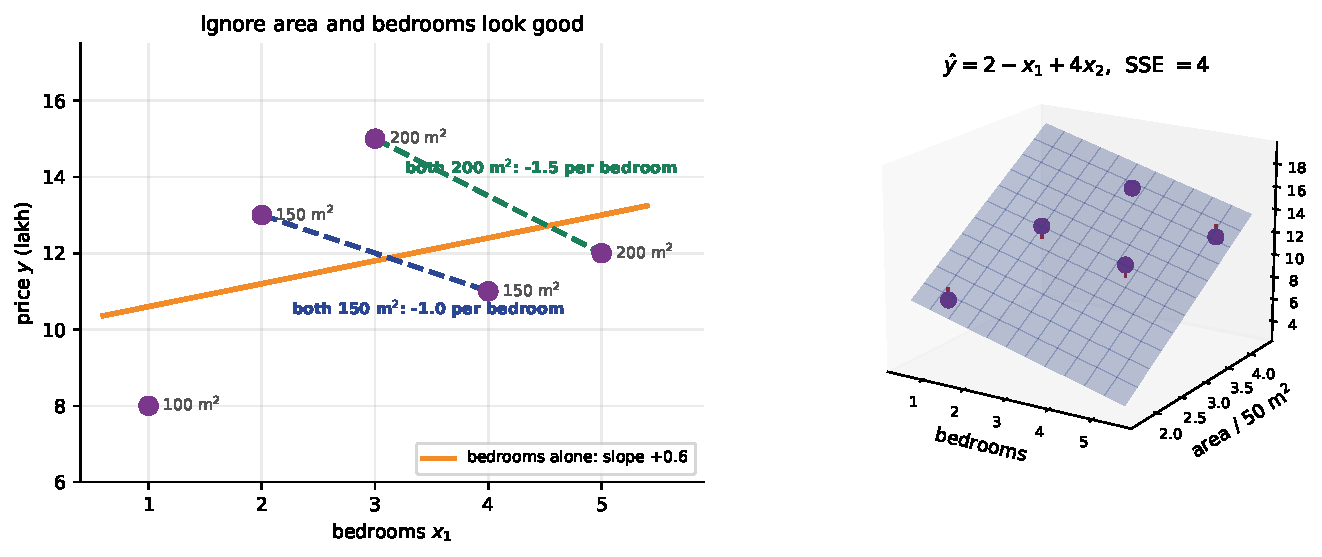
\includegraphics[width=0.84\textwidth]{hand.pdf}
  \caption{Left: price against bedrooms. The orange line, which ignores floor
  area, has slope $+0.6$. The dashed segments join the pairs of flats that
  \emph{share} a floor area, and they go down: $-1.0$ per bedroom at
  $150\,\mathrm{m}^2$, $-1.5$ at $200\,\mathrm{m}^2$. Right: the fitted plane
  $\hat y = 2 - x_1 + 4x_2$, with the five residuals drawn as vertical bars
  whose squares sum to $\mathrm{SSE} = 4$.}
  \label{fig:hand}
\end{figure}

\begin{tryit}
Refit the five flats after \emph{deleting} flat C, whose residual is zero.
The deleted point lies exactly on the fitted plane, so you might expect
nothing to change. Compute $\Xt X$, $\det$, and $\hat\beta$ for the remaining
four rows. You should find that $\hat\beta$ is unchanged at $(2,-1,4)$ ---
deleting a point with zero residual does not move a least-squares fit ---
while $\det(\Xt X)$ drops from $60$ to $12$ and $R^2$ changes because SST
changes.
\end{tryit}

\notesources{\AMLUnitVSources}

% =========================================================================
\section{Interpreting the coefficients}
\label{sec:interp}

\subsection{``Holding the others fixed''}

\begin{keyidea}
$b_j$ is the change in $\hat y$ associated with a one-unit increase in $x_j$
\textbf{when every other predictor in the model is held constant}. The clause
is not decoration. It names the other columns you happened to include, and it
is the reason $b_j$ changes when you change them.
\end{keyidea}

Three things follow immediately, and each of them catches people out.

\paragraph{The coefficient belongs to the model, not to the column.} There is
no such thing as ``the effect of $x_j$''. There is the effect of $x_j$ in
\emph{this} model, with \emph{these} other predictors. Add a column and every
coefficient may move.

\paragraph{The clause may describe an impossible intervention.} ``Holding
total cholesterol fixed, LDL cholesterol has effect $b$'' describes a
manipulation nobody can perform, since LDL is a component of the total. The
number is still well defined and still computable. It simply does not mean
what a newspaper headline would say it means.

\paragraph{The sign can be the opposite of the marginal association.} This is
the subject of the next subsection, and it is the single most important thing
in this lecture.

For the five flats, $b_1 = -1$ does not say that bedrooms make a flat cheaper.
It says: among flats of the \emph{same floor area}, the one chopped into more
bedrooms is worth less --- smaller rooms. Meanwhile the marginal slope
$+0.6$ says: flats with more bedrooms tend to be bigger, and bigger flats cost
more. Both are true, and they are answers to different questions.

\subsection{The sign flip, on real data}
\label{sec:signflip}

\begin{lstlisting}
full = LinearRegression().fit(X, y)
for j, name in enumerate(dia.feature_names):
    simple = LinearRegression().fit(X[:, [j]], y).coef_[0]
    print(name, simple, full.coef_[j])
\end{lstlisting}
\begin{codeout}
feature   simple slope   slope in the full 10-feature model
age            +1.1050                -0.0364  <-- SIGN FLIP
sex            +6.6454               -22.8596  <-- SIGN FLIP
bmi           +10.2331                +5.6030
bp             +2.4607                +1.1168
s1             +0.4723                -1.0900  <-- SIGN FLIP
s2             +0.4412                +0.7465
s3             -2.3531                +0.3720  <-- SIGN FLIP
s4            +25.7158                +6.5338
s5            +83.5114               +68.4831
s6             +2.5649                +0.2801
\end{codeout}

Four of the ten predictors change sign. Take \texttt{s1}, total serum
cholesterol. On its own its slope is $+0.4723$ per mg/dl: more cholesterol,
worse disease progression, which is what everybody expects. Put the other nine
measurements alongside it and the slope becomes $-1.0900$: the opposite sign,
and $2.31$ times the magnitude.

\begin{caution}
Ten simple regressions are not one multiple regression, and no amount of care
in running them makes them one. A simple slope absorbs the effect of
everything correlated with that column; a multiple slope has had those effects
removed. Reporting a table of simple slopes and describing it as ``the effect
of each variable'' is the commonest error in applied regression, and it is
wrong by more than a factor of two here, in the wrong direction.
\end{caution}

\begin{figure}[tb]
  \centering
  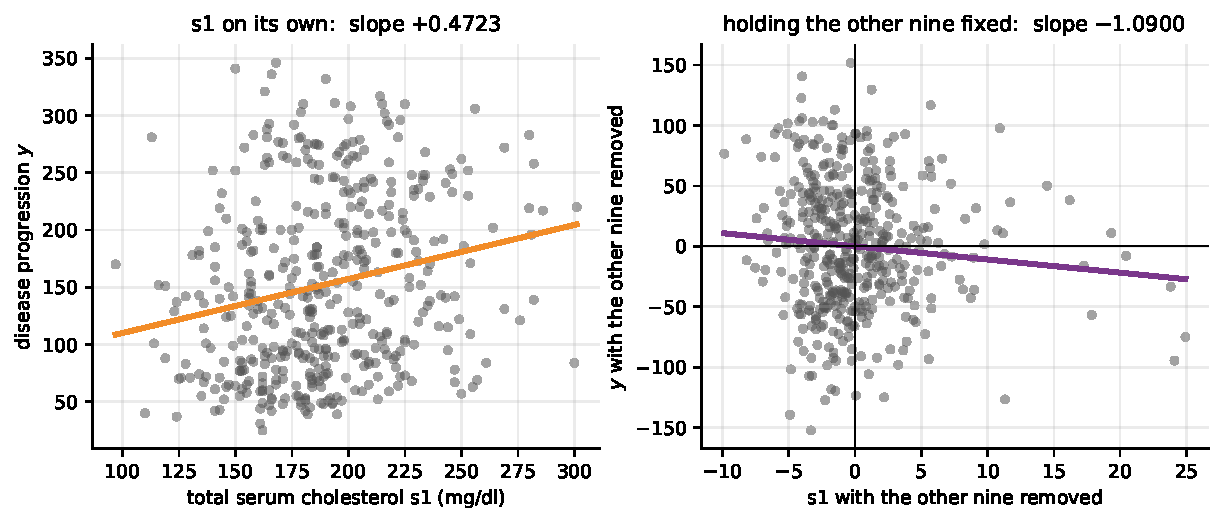
\includegraphics[width=0.76\textwidth]{signflip.pdf}
  \caption{Left: raw \texttt{s1} against disease progression for all $442$
  patients, with the simple regression line of slope $+0.4723$. Right: the
  \emph{added-variable plot} for \texttt{s1}. Both axes have had the other
  nine predictors regressed out, and the remaining relationship slopes
  \emph{down}, at exactly the multiple-regression coefficient $-1.0900$. Same
  patients, same column, opposite conclusion.}
  \label{fig:signflip}
\end{figure}

\subsection{Where the difference goes: the omitted-variable formula}
\label{sec:ovb}

Suppose the true model has two predictors but you fit only the first. Write
$b_1, b_2$ for the coefficients in the two-predictor fit and $\delta$ for the
slope of $x_2$ regressed on $x_1$. Then
\begin{equation}
  \label{eq:ovb}
  b_1^{\text{simple}} = b_1 + b_2\,\delta .
\end{equation}
In words: the simple slope is the partial slope \emph{plus} whatever effect
$x_1$ borrows from $x_2$ by being correlated with it. The borrowed term is
large when $x_2$ matters a lot ($b_2$ large) and when the two predictors move
together ($\delta$ large).

\begin{lstlisting}
pair  = LinearRegression().fit(X[:, [i_s1, i_s5]], y)
delta = LinearRegression().fit(X[:, [i_s1]], X[:, i_s5]).coef_[0]
print(pair.coef_[0] + pair.coef_[1] * delta)
\end{lstlisting}
\begin{codeout}
s1 (total cholesterol) alone            +0.4723
s1 with s5 (log triglycerides) added    -0.2418
s5 in that pair                         +91.7683
corr(s1, s5) +0.5155    corr(s1, y) +0.2120    corr(s5, y) +0.5659

the omitted-variable formula: b_simple = b_partial + b_s5 * delta
   regress s5 on s1: delta = +0.007781
   -0.2418 + +91.7683 * +0.007781 = +0.4723   (simple slope +0.4723)
\end{codeout}

The identity holds to four decimal places, as it must --- it is algebra, not
an approximation. The borrowed term is $91.7683 \times 0.007781 = 0.714$, and
$-0.2418 + 0.714 = +0.4723$. \textbf{Two predictors are enough to flip the
sign; adding the other eight takes it from $-0.24$ to $-1.09$.}

\begin{keyidea}
A coefficient changes when you add a predictor if and only if the new
predictor is correlated with the old one \emph{and} with the target. If either
correlation is zero, nothing moves. This is why designed experiments randomise
--- randomisation makes $\delta = 0$ in expectation and the simple slope is
then already the partial one.
\end{keyidea}

\subsection{Partial regression coefficients and added-variable plots}
\label{sec:fwl}

There is a second, constructive definition of $b_j$ that never mentions the
other coefficients:

\begin{enumerate}[leftmargin=*]
  \item Regress $x_j$ on all the \emph{other} predictors and keep the residual
    $\tilde x_j$. This is the part of $x_j$ that nothing else in the model
    explains.
  \item Regress $y$ on all the other predictors and keep the residual
    $\tilde y$.
  \item Regress $\tilde y$ on $\tilde x_j$. The single slope you get is
    $b_j$ --- exactly, not approximately.
\end{enumerate}

This is the \textbf{Frisch--Waugh--Lovell} theorem, and the quantity it
produces is what the syllabus calls the \textbf{partial regression
coefficient}. It is the precise content of ``holding the others fixed'': both
variables have had the other predictors' influence subtracted before they are
compared.

\begin{lstlisting}
others = [k for k in range(X.shape[1]) if k != j]
ex = X[:, j] - LinearRegression().fit(X[:, others], X[:, j]).predict(X[:, others])
ey = y       - LinearRegression().fit(X[:, others], y      ).predict(X[:, others])
print(LinearRegression().fit(ex.reshape(-1, 1), ey).coef_[0])
\end{lstlisting}
\begin{codeout}
residual of s1 after regressing it on the other nine   sd 4.4979
residual of y  after regressing it on the other nine   sd 53.7607
slope of (y residual) on (s1 residual)  -1.0899963341
coefficient of s1 in the full model     -1.0899963341
difference 2.15e-14

corr(s1 residual, s1) 0.1300  -- only 1.7% of s1's variance is its own
\end{codeout}

The scatter of $\tilde y$ against $\tilde x_j$ is the \textbf{added-variable
plot} (also called a partial regression plot). It is the only honest
two-dimensional picture of a multiple-regression coefficient, and it tells you
three things at once: the slope is $b_j$; the horizontal spread shows how much
independent information $x_j$ carries; and outliers and curvature that the
raw scatter hides become visible.

\begin{figure}[tb]
  \centering
  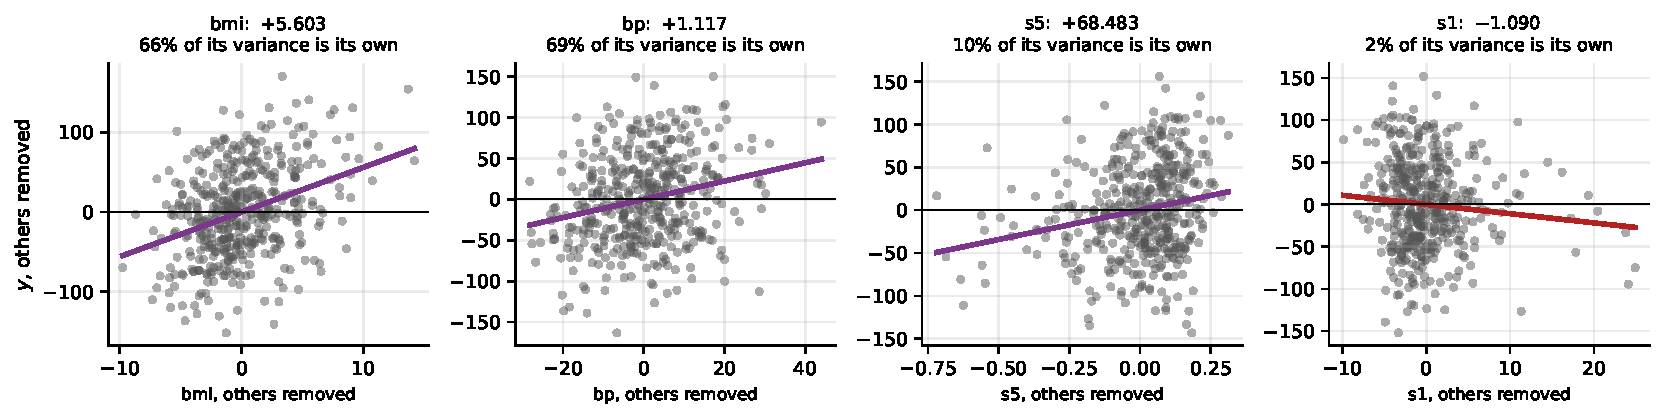
\includegraphics[width=0.94\textwidth]{avplot.pdf}
  \caption{Added-variable plots for four of the ten diabetes predictors. The
  slope of each cloud \emph{is} the coefficient in the ten-predictor model.
  The second line of each title is the fraction of that predictor's variance
  that survives regression on the other nine: $66\%$ for \texttt{bmi},
  $69\%$ for \texttt{bp}, $9.9\%$ for \texttt{s5} and only $1.7\%$ for
  \texttt{s1}. The narrower the horizontal spread, the less the data has to
  say about that coefficient.}
  \label{fig:avplot}
\end{figure}

\begin{keyidea}
Only $1.7\%$ of \texttt{s1}'s variance is its own. Its coefficient is
estimated from that $1.7\%$ and from nothing else. That single number
predicts everything in Section~\ref{sec:mc}.
\end{keyidea}

\notesources{\AMLUnitVSources}

% =========================================================================
\section{Standardized (beta) coefficients}
\label{sec:std}

\subsection{Why raw coefficients cannot be compared}

$b_j$ has units of $y$ per unit of $x_j$. Two coefficients whose denominators
are different units are not the same kind of number, and ranking them by
magnitude ranks the units, not the predictors. In the diabetes model the
largest raw coefficient is $\texttt{s5} = +68.48$ --- but \texttt{s5} is a
logarithm with a standard deviation of $0.52$, while \texttt{s1} is in mg/dl
with a standard deviation of $34.6$. A one-unit change means something
completely different in the two columns.

The fix is to put both sides in standard-deviation units. Replacing $x_j$ by
$(x_j - \bar x_j)/s_j$ divides that column by $s_j$ and therefore multiplies
its coefficient by $s_j$; replacing $y$ by $(y-\bar y)/s_y$ divides every
coefficient by $s_y$. So
\begin{equation}
  \label{eq:betastar}
  \beta^*_j = b_j\,\frac{s_j}{s_y} ,
\end{equation}
the \textbf{standardized} or \textbf{beta} coefficient: the change in $y$, in
standard deviations of $y$, per one standard deviation of $x_j$, holding the
others fixed. It is dimensionless, and therefore comparable across predictors.

\subsection{Measured, and the ranking changes}

\begin{lstlisting}
sd = X.std(axis=0, ddof=1)
beta_star = full.coef_ * sd / y.std(ddof=1)
\end{lstlisting}
\begin{codeout}
feature    raw coef        sd      beta*   rank raw   rank beta*
s1           -1.0900   34.6081    -0.4893        6            1
s5          +68.4831    0.5224    +0.4640        1            2
bmi          +5.6030    4.4181    +0.3211        4            3
s2           +0.7465   30.4131    +0.2945        7            4
bp           +1.1168   13.8313    +0.2004        5            5
sex         -22.8596    0.4996    -0.1481        2            6
s4           +6.5338    1.2904    +0.1094        3            7
s3           +0.3720   12.9342    +0.0624        8            8
s6           +0.2801   11.4963    +0.0418        9            9
age          -0.0364   13.1090    -0.0062       10           10

largest by raw magnitude  : s5 (+68.4831)
largest by beta*          : s1 (-0.4893)
\end{codeout}

\texttt{s1} moves from sixth by raw magnitude to \textbf{first} by $\beta^*$;
\texttt{sex} moves from second to sixth. The raw ranking was a ranking of
measurement units.

The unit-free claim is checkable. Record \texttt{bmi} in units of
$10^{-4}\,\mathrm{kg/m^2}$ --- the same data, multiplied by $10^4$ --- and
refit:

\begin{codeout}
   bmi coefficient  +5.6030  (kg/m2)   +0.00056030  (1e-4 kg/m2)
   beta* for bmi    +0.321100  and  +0.321100   -- unchanged
check against a regression on standardised columns: max diff 7.72e-15
\end{codeout}

The raw coefficient changed by a factor of $10^4$; $\beta^*$ did not change at
all. And rescaling by $s_j/s_y$ gives exactly the same numbers as putting a
\texttt{StandardScaler} in front of the regression, to $7.7\times10^{-15}$.

\begin{figure}[tb]
  \centering
  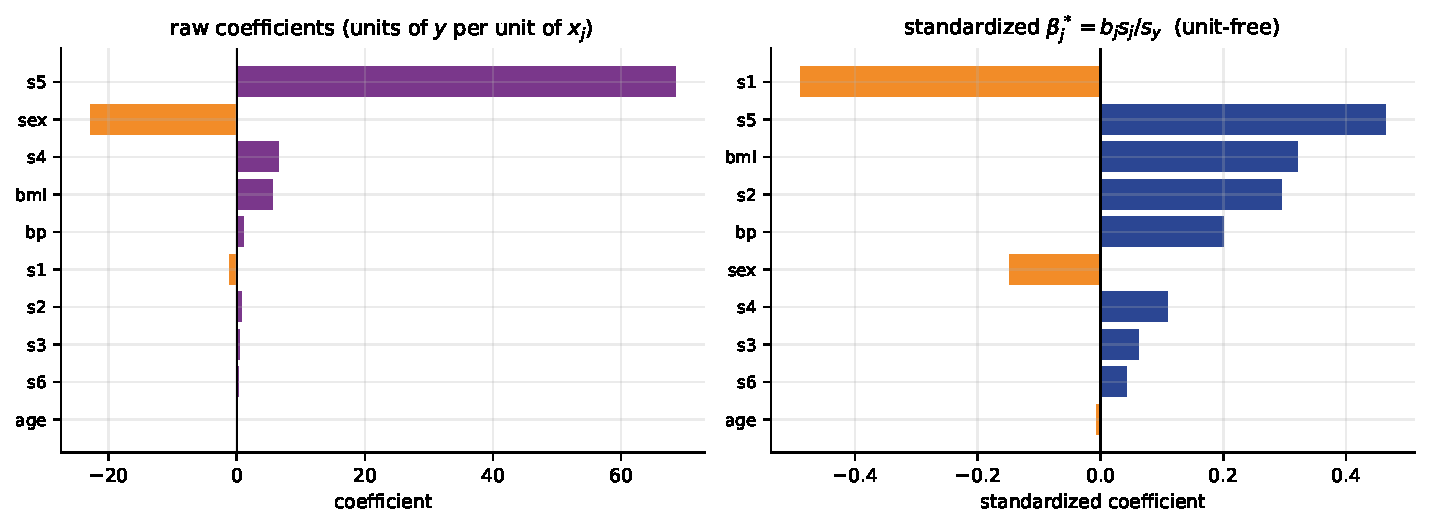
\includegraphics[width=0.84\textwidth]{stdcoef.pdf}
  \caption{Left: the raw coefficients of the ten-predictor diabetes model,
  sorted by magnitude. One bar dwarfs the rest and it tells you only that
  \texttt{s5} is recorded in small numbers. Right: the same fit, standardized.
  Five predictors now sit within a factor of two of each other and
  \texttt{s1} has come first.}
  \label{fig:stdcoef}
\end{figure}

\begin{caution}
$\beta^*$ solves the units problem and nothing else. It is still conditional
on the other predictors; it still inherits any instability from
multicollinearity; and $s_j$ is estimated from \emph{this} sample, so a
predictor with an unusually wide spread in your data will look important.
$\beta^*$ ranks; it does not adjudicate, and it certainly does not establish
causation.
\end{caution}

\begin{tryit}
Fit the wine table: predict \texttt{proline} from \texttt{alcohol},
\texttt{flavanoids} and \texttt{color\_intensity}. You should get
$R^2 = 0.5471$, adjusted $R^2 = 0.5393$, raw coefficients
$(+187.07, +126.41, +16.54)$ and
$\beta^* = (0.4823, 0.4010, 0.1217)$. Note that here the raw and standardized
rankings \emph{agree} --- the three columns happen to have comparable spreads.
Standardizing is not always dramatic; it is always safe.
\end{tryit}

\notesources{\AMLUnitVSources}

% =========================================================================
\section{Multicollinearity}
\label{sec:mc}

\subsection{Near-dependence, and what it costs}

Section~\ref{sec:rank} dealt with \emph{exact} dependence, where $\Xt X$ is
singular. The practically important case is \emph{near} dependence: $\Xt X$ is
invertible, so everything runs, but the inverse is enormous and the
coefficients are estimated from very little information.

The relevant quantity is how well each predictor can be reconstructed from the
others. Let $R_j^2$ be the $R^2$ from regressing $x_j$ on all the other
predictors. Then the variance of the estimated coefficient is
\begin{equation}
  \label{eq:vif}
  \operatorname{Var}(\hat\beta_j) =
  \frac{\sigma^2}{(n-1)s_j^2}\cdot\frac{1}{1-R_j^2},
  \qquad
  \mathrm{VIF}_j = \frac{1}{1-R_j^2}.
\end{equation}
The first factor is what you would get if the predictors were orthogonal. The
second, the \textbf{variance inflation factor}, is the price of collinearity.
Standard errors --- which are square roots of variances --- are multiplied by
$\sqrt{\mathrm{VIF}_j}$.

\begin{worked}[Reading a VIF]
$R_j^2 = 0$ gives $\mathrm{VIF} = 1$: no inflation. $R_j^2 = 0.5$ gives $2$.
$R_j^2 = 0.9$ gives $10$, so a standard error $\sqrt{10} = 3.2$ times larger.
$R_j^2 = 0.99$ gives $100$ and a standard error ten times larger --- which
means you need $100$ times as many observations to estimate that coefficient
as precisely as an uncorrelated one.

The conventional thresholds are $\mathrm{VIF} > 5$ ``look into it'' and
$\mathrm{VIF} > 10$ ``there is a problem''. They are conventions, not
theorems. What matters is whether the coefficient you intend to
\emph{interpret} is one of the inflated ones.
\end{worked}

\begin{lstlisting}
def vif(A):
    out = []
    for j in range(A.shape[1]):
        o = [k for k in range(A.shape[1]) if k != j]
        rj2 = LinearRegression().fit(A[:, o], A[:, j]).score(A[:, o], A[:, j])
        out.append(1.0 / (1.0 - rj2))
    return np.array(out)
\end{lstlisting}
\begin{codeout}
feature      R2_j      VIF   sqrt(VIF)
s1         0.9831    59.20     7.69
s2         0.9745    39.19     6.26
s3         0.9351    15.40     3.92
s5         0.9008    10.08     3.17
s4         0.8875     8.89     2.98
bmi        0.3375     1.51     1.23
s6         0.3264     1.48     1.22
bp         0.3148     1.46     1.21
sex        0.2176     1.28     1.13
age        0.1785     1.22     1.10

rule of thumb: VIF > 5 is worth a look, VIF > 10 is a problem
here 4 of the 10 exceed 10

drop s1 (the worst) and refit:
   s4       VIF     7.82
   s3       VIF     3.74
   s2       VIF     2.93
   s5       VIF     2.17
\end{codeout}

$98.31\%$ of \texttt{s1} is predictable from the other nine columns --- which
is the same fact as ``only $1.7\%$ of its variance is its own'' from
Section~\ref{sec:fwl}, seen from the other side. Its standard error is $7.69$
times what it would be if the columns were orthogonal. And the structure is no
mystery: \texttt{s4} is \texttt{s1}/\texttt{s3} by definition and \texttt{s2}
is part of \texttt{s1}. Dropping \texttt{s1} alone takes the worst remaining
VIF from $59.2$ to $7.8$.

\begin{figure}[tb]
  \centering
  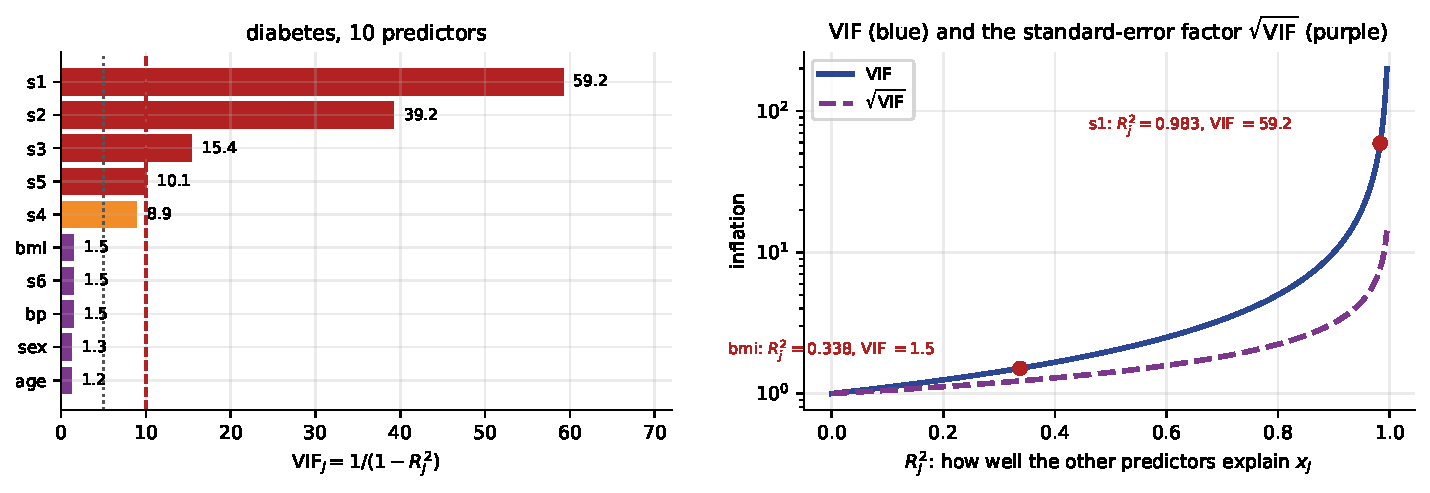
\includegraphics[width=0.90\textwidth]{vif.pdf}
  \caption{Left: the ten variance inflation factors, with the conventional
  thresholds at $5$ (dotted) and $10$ (dashed). Right: the curve
  $\mathrm{VIF} = 1/(1-R_j^2)$ on a logarithmic axis, together with the
  standard-error factor $\sqrt{\mathrm{VIF}}$. The curve is nearly flat until
  $R_j^2 \approx 0.8$ and then goes vertical, which is why collinearity tends
  to arrive suddenly rather than gradually.}
  \label{fig:vif}
\end{figure}

\subsection{Coefficient instability, measured by the bootstrap}
\label{sec:boot}

A VIF is a prediction about variance. The bootstrap measures it directly:
resample the $442$ patients with replacement, refit, and look at the spread of
the coefficients across $2000$ resamples. Each resample is a plausible
alternative dataset from the same population.

\begin{lstlisting}
BOOTSTRAPS = range(0, 2000)      # a sweep: 2000 resamples, one seed each,
                                 # derived from the lecture seed 0
for b, bseed in enumerate(BOOTSTRAPS):
    s = np.random.default_rng(bseed).integers(0, len(X), len(X))
    m = LinearRegression().fit(X[s], y[s])
    coef[b] = m.coef_
    pred[b] = m.predict(X.mean(axis=0).reshape(1, -1))[0]
\end{lstlisting}
\begin{codeout}
2000 bootstrap resamples of the 442 patients
feature    coef    boot sd    2.5%      97.5%     VIF   sign flips
s1         -1.090    0.565    -2.093    +0.113    59.2      3.8%
s2         +0.746    0.512    -0.325    +1.634    39.2      8.6%
s5        +68.483   14.982   +39.101   +97.225    10.1      0.0%
bmi        +5.603    0.721    +4.159    +6.996     1.5      0.0%
bp         +1.117    0.221    +0.680    +1.545     1.5      0.0%

correlation between the bootstrap s1 and s2 coefficients: -0.9637

prediction at the mean patient
   full 10-feature model  mean 152.0573  boot sd 2.5635
   with s1 dropped        mean 152.0647  boot sd 2.5818
   bmi coefficient        boot sd 0.7212 (full) vs 0.7374 (s1 dropped)
\end{codeout}

Read the intervals. \texttt{bmi}, with $\mathrm{VIF} = 1.5$, has a $95\%$
bootstrap interval of $[+4.16, +7.00]$: nowhere near zero, and its sign never
changed in $2000$ resamples. \texttt{s1} has $[-2.09, +0.11]$ and \texttt{s2}
has $[-0.33, +1.63]$: \textbf{both straddle zero}. The fitted \texttt{s2}
coefficient is positive, yet it came out \emph{negative} in one resample out
of twelve; the fitted \texttt{s1} coefficient is negative, yet it came out
positive in about one in twenty-six. Neither sign is established by $442$
patients.

The correlation of $-0.964$ between the two bootstrap coefficients is the
mechanism made visible. \texttt{s1} and \texttt{s2} are nearly the same
column, so the data determines their \emph{sum} well and the split between
them hardly at all. Every resample slides the pair along a line.

\begin{figure}[tb]
  \centering
  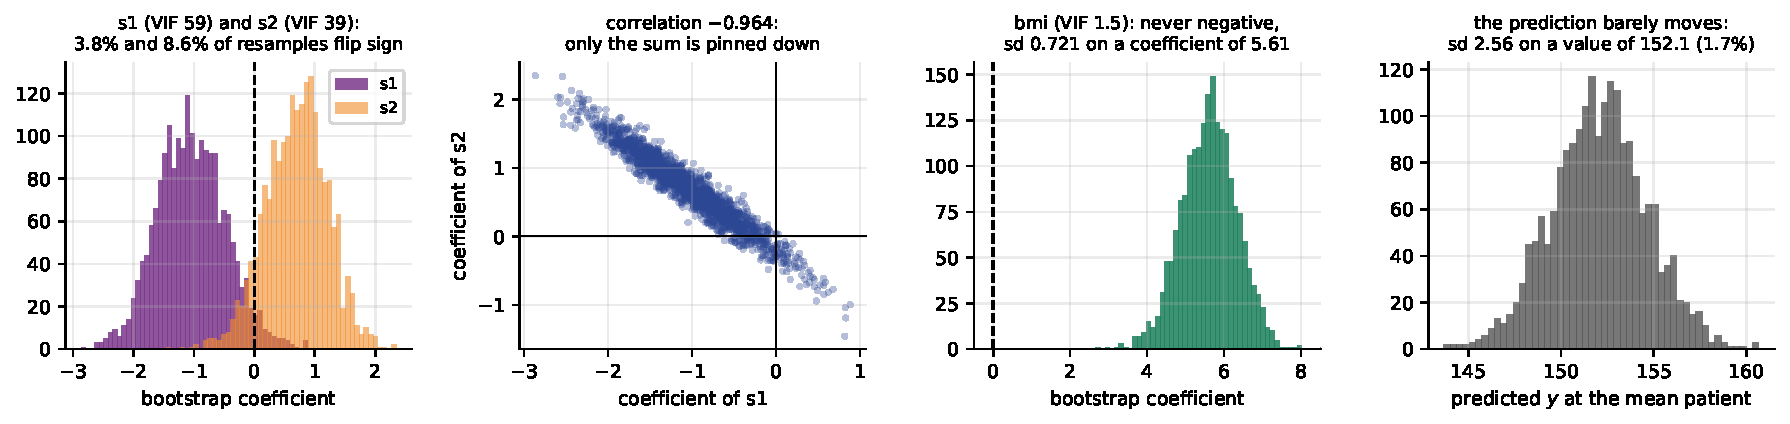
\includegraphics[width=0.98\textwidth]{boot.pdf}
  \caption{$2000$ bootstrap resamples. Panels 1 and 2: the \texttt{s1} and
  \texttt{s2} coefficients are individually uncertain and jointly almost
  perfectly anti-correlated --- their sum is pinned down and the split is not.
  Panel 3: \texttt{bmi}, with $\mathrm{VIF} = 1.5$, is never negative. Panel
  4: the prediction at the mean patient has a standard deviation of $1.7\%$ of
  its value, while the coefficients producing it are barely determined.}
  \label{fig:boot}
\end{figure}

\subsection{Predicting is fine. Explaining is not.}
\label{sec:predexp}

This is the distinction the whole section exists for. Take two predictors
correlated at $0.9986$, generated so that the truth is
$y = 3x_1 + 2x_2 + \varepsilon$. Fit on the first hundred rows, then on the
second hundred.

\begin{codeout}
corr(a, b) 0.9986    true coefficients 3.0 and 2.0     VIF [351.6 351.6]
fitted on all 200 rows: +2.438  +2.595  (sum +5.034, truth 5.000)
first half   a   +2.553  b   +2.460   sum  +5.012   test R2 +0.9895
second half  a   +2.208  b   +2.848   sum  +5.056   test R2 +0.9895
the two coefficient vectors differ by 0.39, their sum by 0.044
\end{codeout}

Read the individual coefficients against the truth. The generating values
were $b_1 = 3$ and $b_2 = 2$, and \textbf{not one of the three fits recovers
them}: on all $200$ rows least squares reports $(+2.44, +2.60)$, and the two
halves report $(+2.55, +2.46)$ and $(+2.21, +2.85)$. The estimates wander over
a range of about $0.4$ from one half of the data to the other, and they sit
roughly half a unit from the truth in opposite directions.

Now read the sum. It is $5.034$, $5.012$ and $5.056$ against a truth of
$5.000$ --- \textbf{agreeing to about four parts in a thousand while the
individual coefficients are simply wrong}. Both halves score
$R^2 = 0.9895$ on the same evaluation data, identical to four decimal places,
and their predictions correlate at $r = 0.99999$.

That is the whole lesson in one table: what the data constrains here is
$b_1 + b_2$, and the split between the two is decided by noise. Be careful not
to over-claim it. On this particular sample the two halves do \emph{not}
disagree about the \emph{sign} of $b_2$ --- both are positive. Collinearity
does not guarantee a sign flip; it guarantees that the split is unreliable,
and a sign flip is simply what that unreliability looks like when the
coefficient is close enough to zero. For sign flips that really did happen,
look back at the real diabetes table in Section~\ref{sec:signflip}, where
four of ten coefficients change sign, and at the bootstrap above, where
\texttt{s2} flips in $8.6\%$ of resamples.

The same point on the real table:

\begin{codeout}
cross-validated R2, all 10 features        +0.4892
cross-validated R2, s1 dropped             +0.4867
cross-validated R2, s1 and s2 both dropped +0.4867
cross-validated R2, ridge(alpha=1) on standardised columns +0.4896

ridge coefficients are stable where least squares is not:
   feature   OLS (standardised)   ridge
   s1               -37.6800  -30.0884
   s2               +22.6762  +16.6532
   s5               +35.7344  +32.8438
   bmi              +24.7265  +24.7712
\end{codeout}

Dropping the two worst-behaved predictors costs $0.0025$ of cross-validated
$R^2$ --- nothing.

\begin{keyidea}
Multicollinearity is a disease of the coefficients, not of the predictions. If
all you need is $\hat y$, you may ignore it entirely. If anybody is going to
read a coefficient, write it in a report, or make a decision from its sign,
you may not.
\end{keyidea}

\begin{figure}[tb]
  \centering
  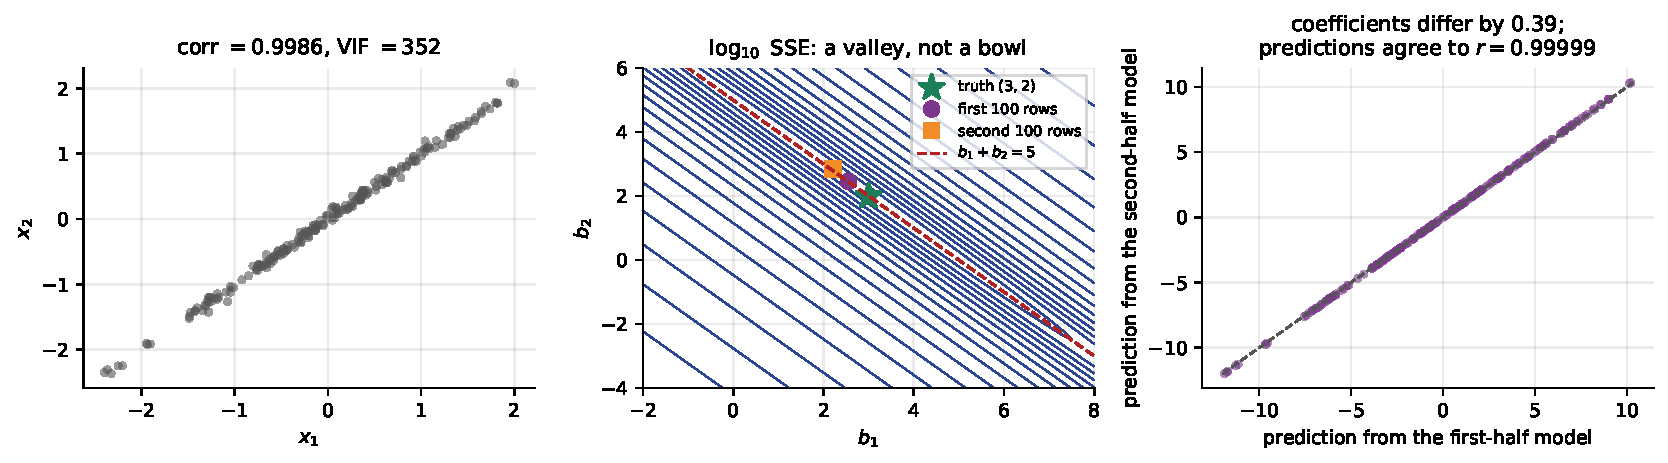
\includegraphics[width=0.94\textwidth]{collinear.pdf}
  \caption{Left: two predictors correlated at $0.9986$, $\mathrm{VIF} = 352$.
  Middle: the residual sum of squares as a function of $(b_1, b_2)$. It is a
  long trench along $b_1 + b_2 = 5$ rather than a bowl, so which point in the
  trench you land on is decided by noise; the purple circle and orange square
  are the two half-samples. Right: their predictions nevertheless agree to
  $r = 0.99999$.}
  \label{fig:collinear}
\end{figure}

\subsection{What to do about it}

\begin{center}
\begin{tabular}{@{}lp{4.9cm}p{5.0cm}@{}}
\toprule
& \textbf{What it does} & \textbf{What it costs}\\
\midrule
\textbf{Nothing} & entirely acceptable if the model is only ever used to
  predict & no coefficient may be interpreted, and you must say so\\[4pt]
\textbf{Drop a column} & removes the redundancy; VIFs fall immediately &
  the survivor now carries both effects, so the choice of which to keep is a
  scientific decision, not a statistical one\\[4pt]
\textbf{Combine columns} & replace \texttt{s1} and \texttt{s2} by a sum, a
  ratio or an index & you must be able to name and defend the combination\\[4pt]
\textbf{Ridge or lasso} & $\Xt X + \lambda I$ is invertible for every
  $\lambda>0$, and the coefficients stabilise &
  the estimates are biased; $\lambda$ must be chosen by cross-validation
  (next lecture)\\[4pt]
\textbf{More data} & shrinks every standard error by $\sqrt{n}$ &
  useless when the columns are collinear \emph{by definition}, as
  \texttt{s4} $=$ \texttt{s1}/\texttt{s3} is\\
\bottomrule
\end{tabular}
\end{center}

Note what is \emph{not} on that list: dropping a predictor because its
$p$-value is large. In a collinear pair both $p$-values are large precisely
because the two are fighting over the same information, and dropping either
one makes the other significant.

\notesources{\AMLUnitVSources}

% =========================================================================
\section{Missing data in a regression}
\label{sec:missing}

\subsection{Why it is worse here than you expect}

Least squares needs a complete row. One missing cell in one column removes the
entire observation from the fit, and with $d$ columns each missing
independently at rate $p$, a row survives with probability $(1-p)^d$. That
exponent is the whole problem.

\begin{center}
\begin{tabular}{@{}rrr@{}}
\toprule
$p$ & rows kept of $309$ ($d=10$) & fraction\\
\midrule
$0.01$ & $279$ & $90.4\%$\\
$0.02$ & $252$ & $81.7\%$\\
$0.05$ & $185$ & $59.9\%$\\
$0.10$ & $108$ & $34.9\%$\\
$0.20$ & $\phantom{0}33$ & $10.7\%$\\
$0.30$ & $\phantom{00}9$ & $\phantom{0}2.8\%$\\
\bottomrule
\end{tabular}
\end{center}

A $10\%$ per-cell missing rate --- which nobody would describe as a serious
data quality problem --- deletes two thirds of the patients, silently.

The earlier data-cleaning lecture introduced the three missingness mechanisms
and they carry over unchanged. Under \textbf{MCAR} the complete cases are a
fair random sample, so you lose precision but not correctness. Under
\textbf{MAR} the complete cases are biased, but the observed columns contain
enough information to undo it --- which is exactly what a regression-based
imputer does. Under \textbf{MNAR} the missingness depends on the unobserved
value itself and no purely computational fix repairs it.

\subsection{Five strategies, measured}

$309$ training rows, ten predictors, MCAR missingness imposed on the training
columns only, evaluated on a held-out third that is complete.

\begin{lstlisting}
from sklearn.experimental import enable_iterative_imputer
from sklearn.impute import SimpleImputer, IterativeImputer
Pipeline([("imp", SimpleImputer(strategy="mean")),
          ("lr",  LinearRegression())]).fit(X_missing, y_train).score(X_test, y_test)
\end{lstlisting}
\begin{codeout}
no missingness at all                test R2 +0.3929

MCAR at 10%: cells missing 10.4%, complete rows 103 of 309 (33.3%)
   listwise deletion            103 rows   test R2 +0.3231
   mean imputation              309 rows   test R2 +0.3875
   median imputation            309 rows   test R2 +0.3850
   mean + missing indicators    309 rows   test R2 +0.3657
   IterativeImputer (MICE)      309 rows   test R2 +0.3871

MCAR at 25%: cells missing 25.2%, complete rows 13 of 309 (4.2%)
   listwise deletion             13 rows   test R2 -2.1451
   mean imputation              309 rows   test R2 +0.4048
   median imputation            309 rows   test R2 +0.3990
   mean + missing indicators    309 rows   test R2 +0.3526
   IterativeImputer (MICE)      309 rows   test R2 +0.4038
\end{codeout}

At $10\%$ listwise deletion already loses $0.0698$ of test $R^2$ against the
complete table, while every imputer recovers most of it. At $25\%$ listwise
deletion leaves $13$ rows to estimate $11$ parameters and the result is
$\mathbf{-2.15}$ --- far worse than predicting $\bar y$ for every patient.
Mean imputation, the crudest method available, scores $+0.405$ on the same
data and \texttt{IterativeImputer} $+0.404$, both a little above the
no-missingness baseline of $+0.393$.

Do not read anything into the ordering of those last two. The gap between mean
imputation and MICE is $0.0010$, and the gap between either of them and the
complete-data baseline is $+0.0119$ and $+0.0109$, on a single split whose
fold-to-fold spread elsewhere in this lecture is $0.11$. \textbf{These
differences are noise.} What the table does establish, unambiguously, is the
size of the effect that matters: throwing rows away costs you $2.5380$ of $R^2$,
and any imputer at all costs you nothing measurable.

\begin{figure}[tb]
  \centering
  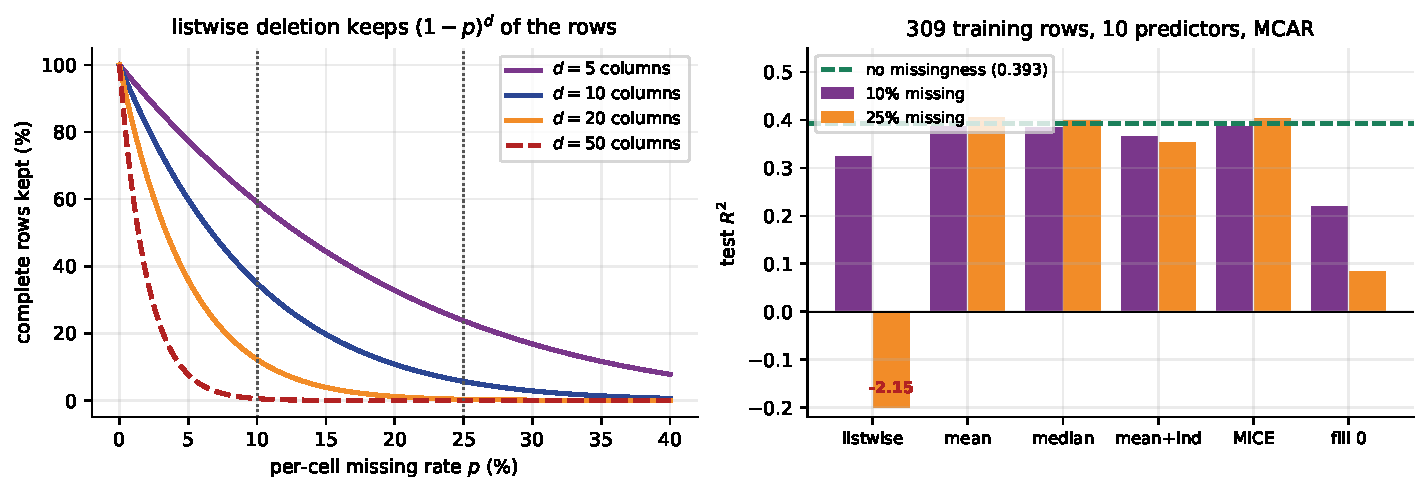
\includegraphics[width=0.84\textwidth]{missing.pdf}
  \caption{Left: the fraction of complete rows, $(1-p)^d$, for four widths of
  table. At $d = 50$ a $5\%$ cell rate keeps about a fifth of the rows.
  Right: the five strategies at two missing rates against the no-missingness
  baseline. The listwise bar at $25\%$ is off the bottom of the axis, at
  $-2.15$; ``fill 0'' is the other bad answer.}
  \label{fig:missing}
\end{figure}

\begin{caution}
Filling missing values with $0$ is not a neutral default. A patient with
\texttt{age} $=0$ and \texttt{bp} $=0$ is not a patient with unknown age; it
is a claim about a newborn with no blood pressure, and least squares believes
it. Measured on the diabetes table at $25\%$ missingness: cross-validated
$R^2$ of $+0.061$, against $+0.411$ for mean imputation. Use
\texttt{np.nan} and an imputer, never a sentinel.
\end{caution}

\subsection{Adding a missing-indicator column}

Setting \texttt{add\_indicator=True} on an imputer appends a binary column
per predictor recording whether that cell was imputed. This is the right move when
the \emph{fact} of missingness is informative --- a test that was not ordered
because the patient looked healthy, a question a respondent declined. On this
MCAR data it \emph{hurt}: $+0.3657$ against $+0.3875$ at $10\%$ missing, and
$+0.3526$ against $+0.4048$ at $25\%$. That is exactly what you would expect
once you think about it. Under MCAR the indicator carries no information about
$y$ at all, so each one is a pure-noise column --- and the previous subsection
is about what pure-noise columns do to a fit. Ten of them on $309$ rows is
enough to cost a couple of points of held-out $R^2$.

So: add indicators when you have a reason to believe the \emph{fact} of
missingness is informative, and not otherwise. Report what the experiment
showed rather than the benefit you were hoping for.

\subsection{An imputer is a learned step}

An imputer estimates column means, or fits a regression per column. Those are
numbers learned from data, so they belong inside the cross-validation fold.

\begin{lstlisting}
# wrong: the column means are computed from every row, including test rows
X_filled = SimpleImputer().fit_transform(X)
cross_val_score(LinearRegression(), X_filled, y, cv=5)

# right: refitted on four fifths of the data inside every fold
cross_val_score(Pipeline([("imp", SimpleImputer()),
                          ("lr",  LinearRegression())]), X, y, cv=5)
\end{lstlisting}
\begin{codeout}
25% MCAR on all 442 rows, 5-fold cross-validation
   mean    impute-then-split +0.4114   inside the Pipeline +0.4112   difference +0.0002
   MICE    impute-then-split +0.4434   inside the Pipeline +0.4392   difference +0.0042
   an imputer never looks at y, so there is very little for it to leak
\end{codeout}

\begin{keyidea}
Report the size of a leak honestly. Here it is $+0.0002$ for mean imputation
and $+0.0042$ for MICE --- real but negligible, for the same reason that
scaling and PCA leak very little: neither ever looks at $y$. Put the imputer
in the \texttt{Pipeline} anyway. It costs nothing, and an imputer that
\emph{does} use the target, or a test set small enough for its mean to matter,
is a different story.
\end{keyidea}

\notesources{\AMLUnitVSources}

% =========================================================================
\section{Model validation}
\label{sec:valid}

\subsection{Three questions, three checks}

\begin{center}
\begin{tabular}{@{}p{3.7cm}p{4.2cm}p{5.2cm}@{}}
\toprule
\textbf{Question} & \textbf{Check} & \textbf{What failure looks like}\\
\midrule
Are the assumptions met? & residual plots, normal Q--Q,
  scale--location & curvature; a fan; heavy tails\\[4pt]
Does it generalise? & train against test, or cross-validation &
  a large gap between them\\[4pt]
Is this extra column earning its place? & adjusted $R^2$, held-out $R^2$,
  a partial $F$ test & $R^2$ up while adjusted and held-out $R^2$ go down\\
\bottomrule
\end{tabular}
\end{center}

\subsection{Residual diagnostics}
\label{sec:resid}

\begin{codeout}
diabetes, 10 features, 309 training rows
   train R2 +0.5539   test R2 +0.3929
   train RMSE 52.954  test RMSE 55.652
   residual mean 6.88e-14 (least squares forces this to 0)
   corr(residual, fitted) -5.24e-16 (forced to 0 too)
   Shapiro-Wilk on the residuals: W 0.9959, p 0.6100
   Breusch-Pagan style check: corr(|residual|, fitted) +0.2079, p 0.0002
\end{codeout}

Take those lines one at a time. The residual mean and the residual--fitted
correlation are zero \emph{by construction} (Section~\ref{sec:geometry}) and
carry no information. The Shapiro--Wilk test gives $p = 0.11$: no evidence
against normal residuals. Train and test RMSE agree to within about $5\%$
($52.95$ against $55.65$), which is the ordinary gap between fitting a sample
and predicting a fresh one, not evidence of overfitting at $309\times10$. But
$|e|$ rises with $\hat y$ at $p = 0.0002$: mild \textbf{heteroscedasticity}.
The coefficients remain unbiased; the standard errors do not, and prediction
intervals will be too narrow at the high end.

\begin{figure}[tb]
  \centering
  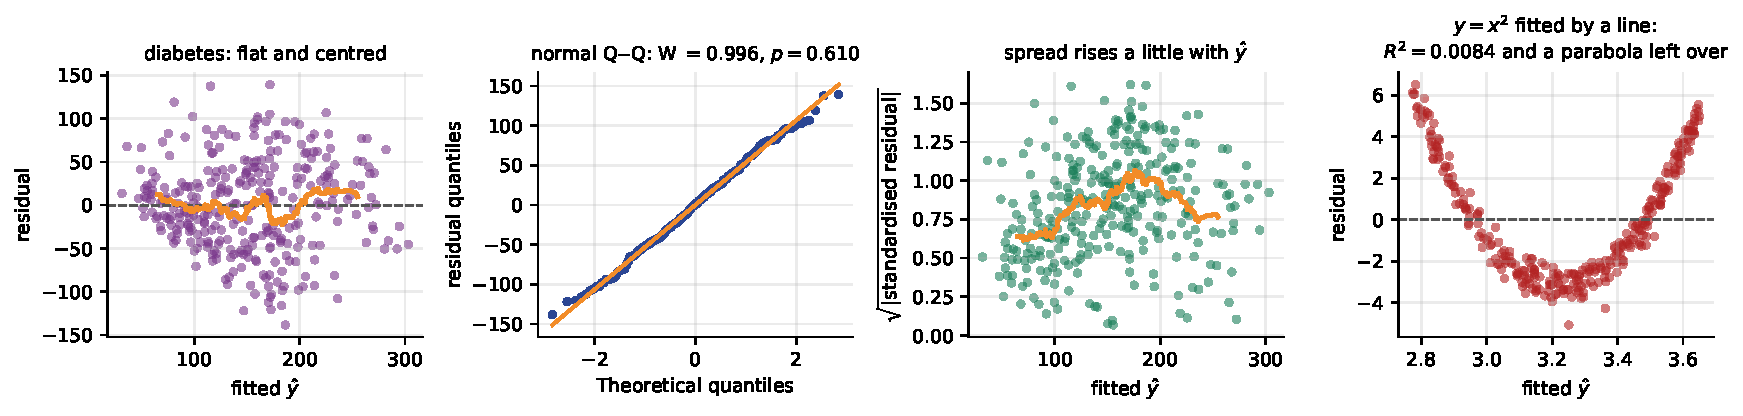
\includegraphics[width=0.98\textwidth]{resid.pdf}
  \caption{The first three panels are the diabetes fit: residuals against
  fitted (flat, with a smoothed trend in orange), a normal Q--Q plot, and a
  scale--location plot showing spread rising slightly with $\hat y$. The
  fourth panel is the point of the figure: $y = x^2 + \varepsilon$ fitted by a
  straight line. $R^2 = 0.0084$, the residual mean is zero, the
  residual--fitted correlation is zero --- and the residual plot is a
  parabola.}
  \label{fig:resid}
\end{figure}

\begin{codeout}
a model that is wrong in a way R2 will not tell you about:
   y = x^2 + noise, fitted with y = b0 + b1 x
   R2 0.0084   residual mean -4.32e-16   corr(residual, fitted) -8.79e-17
   but corr(residual, x^2) +0.9805  -- the plot shows a parabola
   add the x^2 column: R2 0.9710
\end{codeout}

\begin{keyidea}
Every summary statistic on that fit is exactly what a correct model would
produce, and the model is completely wrong. \textbf{Look at the residual
plot.} Adding the one column the picture asks for takes $R^2$ from $0.0084$ to
$0.9710$.
\end{keyidea}

\subsection{\texorpdfstring{$R^2$ always rises; adjusted $R^2$ does not}{R2 always rises; adjusted R2 does not}}
\label{sec:adjr2}

Adding a column can never increase SSE, because the previous solution is still
available with a coefficient of zero. Therefore
\begin{equation}
  \label{eq:monotone}
  R^2 = 1 - \frac{\mathrm{SSE}}{\mathrm{SST}}
  \text{ is monotone non-decreasing in } p,
  \qquad\text{whatever the new column contains.}
\end{equation}
$R^2$ is therefore useless for comparing models of different size. The
standard correction compares mean squares rather than sums:
\begin{equation}
  \label{eq:adj}
  R^2_{\text{adj}} = 1 - \frac{\mathrm{SSE}/(n-p-1)}{\mathrm{SST}/(n-1)}
                   = 1 - (1-R^2)\,\frac{n-1}{n-p-1}.
\end{equation}
A useless column reduces SSE a little and reduces the denominator $n-p-1$ by
one, so the ratio rises and $R^2_{\text{adj}}$ falls. Unlike $R^2$ it can be
negative.

The experiment: $80$ training rows of diabetes, all ten real predictors, then
$k$ columns drawn from $\mathcal{N}(0,1)$ and independent of everything.

\begin{codeout}
adding predictors that are REAL: bmi, then bp, s5, s4, s3 ...
 p   added     train R2   adj R2
 1   bmi          0.4706   0.4639
 2   bp           0.4751   0.4615
 3   s5           0.5481   0.5303
 4   s4           0.5496   0.5256
 5   s3           0.5667   0.5374
 6   s1           0.5751   0.5402

adding predictors that are NOISE: 80 training rows, 10 real features,
then k columns drawn from N(0,1) and independent of everything
 junk k      p   train R2   adj R2    test R2
      0     10     0.5911   0.5318     0.2488
      1     11     0.5992   0.5344     0.2295
      2     12     0.6048   0.5341     0.1939
      3     13     0.6061   0.5285     0.2003
      5     15     0.6183   0.5289     0.1719
      8     18     0.6226   0.5112     0.1571
     10     20     0.6407   0.5188     0.1340
     15     25     0.6502   0.4883     0.0756
     20     30     0.6935   0.5059    -0.0794

train R2 rises at every single step: 8 of 8 increases
adjusted R2 is highest at k = 1, i.e. it is fooled by the first 1 junk column(s) and then falls
test R2 falls at 7 of 8 steps, from +0.2488 to -0.0794
\end{codeout}

Both tables repay reading. With \emph{real} predictors, $R^2$ and
$R^2_{\text{adj}}$ rise together --- until \texttt{s1} joins at $p=6$ and the
adjustment falls, because \texttt{s1} is nearly redundant given \texttt{s3}
and \texttt{s4}. With \emph{noise} predictors, $R^2$ rose at all eight steps,
and held-out $R^2$ fell at seven of the eight, from $+0.249$ all the way to
$\mathbf{-0.079}$ --- past zero, so the model with twenty junk columns is
worse on fresh patients than predicting $\bar y$ for everybody.

Look hard at the middle column, because it is the one that catches people out.
$R^2_{\text{adj}}$ does \emph{not} peak at no junk at all: it rises from
$0.5318$ to $0.5344$ when the first junk column is added, and only then starts
to fall. The adjustment is a fixed arithmetic penalty of
$(n-1)/(n-p-1)$; it knows how many columns you used but nothing whatever about
whether they were real, so a junk column that happens to fit a little noise
can still pay for itself. \textbf{Adjusted $R^2$ can be fooled, and here it
was.}

\begin{codeout}
push it further: k = 60 gives 71 parameters for 80 rows
   train R2 0.9757   test R2 -7.3523   adjusted R2 0.7863
\end{codeout}

\begin{caution}
As $p \to n-1$ the factor $(n-1)/(n-p-1)$ explodes and $R^2_{\text{adj}}$
stops meaning anything: at $71$ parameters on $80$ rows it reads a cheerful
$0.786$ while the held-out $R^2$ is $-7.35$. \textbf{Adjusted $R^2$ is a
warning light, not a model selection criterion.} The criterion is held-out
error.
\end{caution}

\begin{figure}[tb]
  \centering
  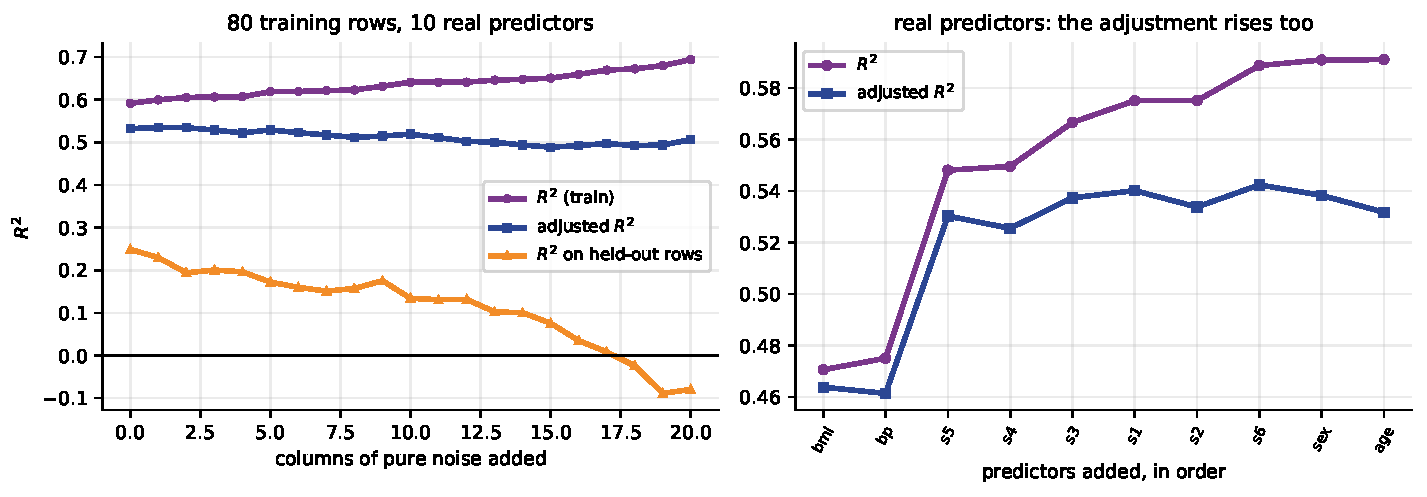
\includegraphics[width=0.84\textwidth]{adjr2.pdf}
  \caption{Left: as pure-noise columns are added to $80$ training rows,
  $R^2$ only ever rises, adjusted $R^2$ drifts down and held-out $R^2$
  collapses. Right: the same three-column arithmetic when the added
  predictors are real --- both curves rise together, and the dip at
  \texttt{s1} and \texttt{s2} is the adjustment noticing two nearly redundant
  columns.}
  \label{fig:adjr2}
\end{figure}

\subsection{Everything in one pipeline}

\begin{lstlisting}
pipe = Pipeline([
    ("imp",   SimpleImputer(strategy="median")),
    ("scale", StandardScaler()),       # so the coefficients are beta*
    ("model", LinearRegression()),
])
cross_val_score(pipe, X, y, cv=KFold(5, shuffle=True, random_state=0))
\end{lstlisting}
\begin{codeout}
impute -> standardise -> least squares, 5-fold on the 10%-missing table
   fold R2 [0.2632 0.3567 0.5213 0.3747 0.5293]
   mean +0.4090  sd 0.1143
   for comparison, the same pipeline on the complete table: +0.4892
\end{codeout}

The column medians and the column means and standard deviations are all
recomputed inside every fold, from four fifths of the data. And read the
fold-to-fold spread: $0.28$ to $0.49$. A single train/test split of $442$
patients would have reported any number in that range with equal confidence,
which is the argument for cross-validating rather than splitting once.

\notesources{\AMLUnitVSources}

% =========================================================================
\section{Summary}

\begin{enumerate}[leftmargin=*]
  \item $y = X\beta + \varepsilon$. Expanding $(y-Xb)^{\!\top}(y-Xb)$ and
    differentiating with the two rules
    $\partial(b^{\!\top}c)/\partial b = c$ and
    $\partial(b^{\!\top}Ab)/\partial b = 2Ab$ gives
    $\nabla S = -2\Xt y + 2\Xt X b$, hence $\Xt X\hat\beta = \Xt y$ and
    $\hat\beta = (\Xt X)^{-1}\Xt y$. The Hessian $2\Xt X$ is positive
    semi-definite, so the stationary point is a global minimum.
  \item $\Xt X$ is invertible exactly when $X$ has full column rank, because
    $\operatorname{null}(\Xt X) = \operatorname{null}(X)$. It fails under
    perfect collinearity and when $p+1 > n$. In both cases
    \texttt{LinearRegression} returns a minimum-norm answer rather than
    raising, and that answer is one of infinitely many.
  \item The five flats, in integers: $\det \Xt X = 60$, the adjugate has rows
    $(266, 22, -100)$, $(22, 14, -20)$ and $(-100, -20, 50)$,
    $\hat\beta = (2,-1,4)$, residuals $(-1,1,0,1,-1)$, $\Xt e = 0$,
    $R^2 = 0.8507$, $R^2_{\text{adj}} = 0.7015$ --- and
    \texttt{LinearRegression} agrees to $8.6\times10^{-14}$.
  \item $b_j$ means ``holding the others fixed''. The bedroom coefficient is
    $-1$ because flats B and D have the same area and differ by two bedrooms
    and two lakh.
  \item \textbf{Total serum cholesterol has slope $+0.4723$ alone and
    $-1.0900$ with nine other predictors in the model}, and four of the ten
    diabetes predictors change sign that way.
  \item The omitted-variable identity accounts for it exactly:
    $-0.2418 + 91.7683\times0.007781 = +0.4723$. A coefficient moves when you
    add a predictor if and only if the new predictor is correlated with both
    the old one and the target.
  \item Frisch--Waugh--Lovell: residualise $x_j$ and $y$ on the other
    predictors and the single slope between the residuals is $b_j$, to
    $2\times10^{-14}$. That scatter is the added-variable plot, and its
    horizontal spread tells you how much the data has to say.
  \item Standardizing changes the ranking. \texttt{s1} goes from sixth by raw
    magnitude to \textbf{first} by $\beta^* = b_j s_j/s_y$, and $\beta^*$ is
    unchanged when \texttt{bmi} is rescaled by $10^4$.
  \item $\mathrm{VIF}_j = 1/(1-R_j^2)$ multiplies
    $\operatorname{Var}(\hat\beta_j)$. Four of the ten diabetes predictors
    exceed $10$; \texttt{s1} reaches $59.2$, so its standard error is
    $7.7\times$ inflated, and only $1.7\%$ of its variance is its own.
  \item $2000$ bootstrap resamples: the \texttt{s1} and \texttt{s2}
    coefficients both straddle zero and correlate at $-0.964$, while the
    prediction at the mean patient varies by $1.7\%$. On a collinear synthetic
    pair whose truth was $(3, 2)$, least squares returned $(+2.44, +2.60)$ and
    the two halves $(+2.55, +2.46)$ and $(+2.21, +2.85)$ --- every one of them
    wrong --- while the sum stayed within $0.06$ of $5$ and the two halves'
    predictions correlated at $0.99999$. \textbf{Collinearity breaks
    explanation, not prediction.}
  \item Missing data: $(1-p)^d$. At $10\%$ across ten columns, two thirds of
    rows are deleted; at $25\%$, listwise deletion scores $-2.15$ while mean
    imputation scores $+0.405$ and MICE $+0.404$ --- a difference between
    those two that is well inside the noise. Filling with $0$ scores
    $+0.061$. The imputer belongs in the \texttt{Pipeline}, though its leak
    here measured only $+0.0002$ to $+0.0042$.
  \item $R^2$ rose at all eight steps as noise columns were added; adjusted
    $R^2$ was fooled by the first one and peaked there, not at zero junk;
    held-out $R^2$ fell from $+0.249$ to $-0.079$. At $71$ parameters on $80$
    rows, adjusted $R^2$ read $0.786$ and held-out $R^2$ was $-7.35$.
    \textbf{Only the held-out number is a criterion.} And a straight line
    fitted to a parabola has $R^2 = 0.0084$, residual mean zero and zero
    residual--fitted correlation: look at the plot.
\end{enumerate}

% =========================================================================
\section{Practice questions}

Attempt these before reading Section~\ref{sec:solutions}. Questions 1, 2, 3, 4
and 6 are hand arithmetic and are the ones most likely to appear on a paper.

\begin{enumerate}[leftmargin=*]
  \item\label{q:derive} Starting from $S(b) = (y - Xb)^{\!\top}(y - Xb)$,
    derive the normal equations. State the two matrix-calculus rules you use
    and verify each by writing out one component. Then show that the
    stationary point is a minimum, and state precisely the condition under
    which the solution is unique.

  \item\label{q:hand} A table has $n = 4$ rows and two predictors:
    $x_1 = (1, 2, 3, 4)$, $x_2 = (1, 3, 2, 4)$ and $y = (5, 15, 14, 20)$.
    (a) Form $\Xt X$ and $\Xt y$. (b) Compute $\det(\Xt X)$ and
    $(\Xt X)^{-1}$ by cofactors. (c) Obtain $\hat\beta$. (d) Verify your
    answer using $\Xt e = 0$. (e) Compute $R^2$ and $R^2_{\text{adj}}$.

  \item\label{q:centred} Repeat question~\ref{q:hand}(c) using the centred
    $2\times2$ system of Equation~\eqref{eq:centred}. Which route would you
    use in an examination with $p = 3$, and why?

  \item\label{q:rank} For each of the following design matrices, state
    whether $\Xt X$ is invertible and give the rank. (a) $n = 100$, $p = 3$,
    all columns distinct and no exact relation. (b) $n = 100$, columns
    ``height in cm'', ``height in inches'', ``weight''. (c) $n = 100$, a
    categorical variable with four levels one-hot encoded into four columns,
    plus an intercept. (d) $n = 12$, $p = 30$. For each case where it fails,
    give the fix and say what \texttt{LinearRegression} will do if you do not
    apply it.

  \item\label{q:ovb} A researcher regresses house price on the number of
    bedrooms and reports a slope of $+0.6$ lakh per bedroom. You then fit
    price on bedrooms and floor area and obtain $-1$ and $+4$. The slope of
    area on bedrooms is $0.4$ (in units of $50\,\mathrm{m}^2$ per bedroom).
    (a) Verify the two results using Equation~\eqref{eq:ovb}. (b) Which
    number should appear in an advertisement for a flat conversion that adds
    a bedroom without extending the building, and why?

  \item\label{q:std} A model predicts monthly household spending in rupees
    from monthly income in rupees ($b = 0.42$, $s_j = 30{,}000$) and from
    household size in persons ($b = 3200$, $s_j = 1.8$). The standard
    deviation of spending is $18{,}000$. (a) Compute both standardized
    coefficients. (b) Which predictor is more important, and what exactly
    does your answer mean? (c) The income column is re-expressed in thousands
    of rupees. What happens to $b$, to $s_j$ and to $\beta^*$?

  \item\label{q:vif} In a five-predictor model, regressing $x_3$ on the other
    four gives $R_3^2 = 0.96$. (a) Compute $\mathrm{VIF}_3$ and the factor by
    which the standard error of $\hat\beta_3$ is inflated. (b) By what factor
    would $n$ have to increase to recover the precision you would have had
    with orthogonal predictors? (c) The $95\%$ bootstrap interval for
    $\hat\beta_3$ turns out to be $[-0.4, +2.1]$ while the model's
    cross-validated $R^2$ is a healthy $0.71$. Write the two sentences you
    would put in the report.

  \item\label{q:missing} A clinical table has $n = 500$ patients and $d = 12$
    predictors, each missing independently at $8\%$. (a) How many complete
    rows do you expect? (b) You need $13$ parameters --- comment. (c) The
    missingness in one column is caused by clinicians not ordering an
    expensive test for patients who looked healthy. Classify the mechanism
    and say what it implies. (d) Give the pipeline you would actually run,
    and say why every step is inside it.

  \item\label{q:report} A colleague sends you this paragraph. ``We fitted a
    linear model of hospital readmission on ten clinical variables. $R^2$ was
    $0.62$, up from $0.55$ with five variables, so the larger model is
    better. Total cholesterol had a coefficient of $-1.09$, so lowering
    cholesterol increases readmission risk; this contradicts the medical
    literature and is our most interesting finding. LDL cholesterol has the
    largest coefficient in the model at $+22.7$, so it is the strongest
    predictor. Residuals had mean zero and were uncorrelated with the fitted
    values, confirming the model is well specified.'' Identify every error,
    say what evidence you would demand for each claim, and rewrite the
    paragraph.

  \item\label{q:design} You must build a model of electricity demand for a
    campus from: outdoor temperature, humidity, a temperature--humidity
    index (computed from the first two), hour of day, day of week, number of
    students on campus, and total floor area of buildings in use. Two of
    these columns have $15\%$ missing values. The model will be used both to
    forecast next week's demand \emph{and} to argue in a committee that
    switching off one building would save a stated amount. Design the
    analysis. For each decision cite a measured number from these notes.
\end{enumerate}

% =========================================================================
\section{Solutions}
\label{sec:solutions}

\textbf{1.} Expand
$S(b) = y^{\!\top}y - y^{\!\top}Xb - b^{\!\top}\Xt y + b^{\!\top}\Xt X b$. The
two middle terms are $1\times1$ and transposes of each other, hence equal, so
$S(b) = y^{\!\top}y - 2b^{\!\top}\Xt y + b^{\!\top}\Xt X b$.

Rule one: $b^{\!\top}c = \sum_j b_jc_j$, so
$\partial/\partial b_k = c_k$ and the gradient is $c$. Rule two: for
symmetric $A$, $b^{\!\top}Ab = \sum_j\sum_k b_jA_{jk}b_k$; the terms involving
$b_m$ are $A_{mm}b_m^2$ and $2A_{mk}b_mb_k$ for $k \ne m$, so
$\partial/\partial b_m = 2\sum_kA_{mk}b_k$ and the gradient is $2Ab$. $\Xt X$
is symmetric because $(\Xt X)^{\!\top} = \Xt X$.

Hence $\nabla S = -2\Xt y + 2\Xt Xb$, and $\nabla S = 0$ gives
$\Xt X\hat\beta = \Xt y$.

Minimum: $\nabla^2 S = 2\Xt X$ and $v^{\!\top}\Xt Xv = \|Xv\|^2 \ge 0$, so the
Hessian is positive semi-definite everywhere and $S$ is convex; every
stationary point is a global minimum.

Uniqueness: the solution is unique iff $\Xt X$ is invertible, which by the
argument of Section~\ref{sec:rank} holds iff $\operatorname{null}(X) = \{0\}$,
that is iff $X$ has full column rank $p+1$. If $\|Xv\| = 0$ for some
$v \ne 0$, then $\hat\beta$ and $\hat\beta + v$ give identical fitted values
and identical SSE.

\medskip
\textbf{2.} (a) $\sum x_1 = 10$, $\sum x_2 = 10$, $\sum x_1^2 = 30$,
$\sum x_2^2 = 30$, $\sum x_1x_2 = 1+6+6+16 = 29$, $\sum y = 54$,
$\sum x_1y = 5+30+42+80 = 157$, $\sum x_2y = 5+45+28+80 = 158$. So
\[
  \Xt X = \begin{pmatrix} 4 & 10 & 10\\ 10 & 30 & 29\\ 10 & 29 & 30
          \end{pmatrix},
  \qquad
  \Xt y = \begin{pmatrix} 54\\157\\158\end{pmatrix}.
\]

(b) Cofactors: $A_{11} = 30\cdot30 - 29^2 = 59$,
$A_{12} = -(10\cdot30 - 29\cdot10) = -10$,
$A_{13} = 10\cdot29 - 30\cdot10 = -10$, so
$\det = 4(59) + 10(-10) + 10(-10) = 236 - 200 = 36$. Also
$A_{22} = 4\cdot30 - 100 = 20$, $A_{23} = -(4\cdot29 - 10\cdot10) = -16$,
$A_{33} = 4\cdot30 - 100 = 20$. Hence
\[
  (\Xt X)^{-1} = \frac{1}{36}
  \begin{pmatrix} 59 & -10 & -10\\ -10 & 20 & -16\\ -10 & -16 & 20
  \end{pmatrix}.
\]

(c) $36b_0 = 59(54) - 10(157) - 10(158) = 3186 - 1570 - 1580 = 36$;
$36b_1 = -10(54) + 20(157) - 16(158) = -540 + 3140 - 2528 = 72$;
$36b_2 = -10(54) - 16(157) + 20(158) = -540 - 2512 + 3160 = 108$. So
$\hat\beta = (1, 2, 3)$ and $\hat y = 1 + 2x_1 + 3x_2$.

(d) Fitted values $(6, 14, 13, 21)$, residuals $e = (-1, +1, +1, -1)$.
Then $\sum e_i = 0$, $\sum x_{1i}e_i = -1+2+3-4 = 0$ and
$\sum x_{2i}e_i = -1+3+2-4 = 0$. All three zero, so $\hat\beta$ satisfies the
normal equations.

(e) $\mathrm{SSE} = 4$. $\bar y = 13.5$, so
$\mathrm{SST} = 8.5^2 + 1.5^2 + 0.5^2 + 6.5^2 = 117$. Hence
$R^2 = 1 - 4/117 = 0.9658$ and, with $n-p-1 = 1$,
$R^2_{\text{adj}} = 1 - (4/1)/(117/3) = 1 - 4/39 = 0.8974$. The gap between
the two is large because three parameters on four rows leave one degree of
freedom.

\begin{codeout}
X'X =
 [[ 4 10 10]
 [10 30 29]
 [10 29 30]]
X'y = [ 54 157 158]      det(X'X) = 36
36 * inv(X'X) =
 [[ 59. -10. -10.]
 [-10.  20. -16.]
 [-10. -16.  20.]]
beta = [1. 2. 3.]      fitted [ 6. 14. 13. 21.]
residuals [-1.  1.  1. -1.]      X'e = [0. 0. 0.]
SSE 4.0000  SST 117.0000  R2 0.965812  adj R2 0.897436
LinearRegression agrees to 1.78e-15
\end{codeout}

\medskip
\textbf{3.} $\bar x_1 = \bar x_2 = 2.5$, $\bar y = 13.5$. Centred:
$x_1^c = (-1.5,-0.5,0.5,1.5)$, $x_2^c = (-1.5,0.5,-0.5,1.5)$,
$y^c = (-8.5,1.5,0.5,6.5)$. Then $S_{11} = S_{22} = 2.25+0.25+0.25+2.25 = 5$,
$S_{12} = 2.25 - 0.25 - 0.25 + 2.25 = 4$,
$S_{1y} = 12.75 - 0.75 + 0.25 + 9.75 = 22$, and
$S_{2y} = 12.75 + 0.75 - 0.25 + 9.75 = 23$. The determinant is
$25 - 16 = 9$, so
\[
  b_1 = \frac{5(22) - 4(23)}{9} = \frac{18}{9} = 2,
  \qquad
  b_2 = \frac{-4(22) + 5(23)}{9} = \frac{27}{9} = 3,
\]
and $b_0 = 13.5 - 2(2.5) - 3(2.5) = 13.5 - 12.5 = 1$. The same answer with
far less arithmetic.

For $p = 3$ the centred route inverts a $3\times3$ instead of a $4\times4$,
and a $4\times4$ determinant alone is four $3\times3$ determinants. Always
centre. The only cost is one extra line for the intercept.

\begin{codeout}
centred cross-product matrix [[5.0, 4.0], [4.0, 5.0]]   det 8.999999999999998
centred X'y [22. 23.]
slopes [2. 3.]   intercept 1.0
\end{codeout}

\medskip
\textbf{4.} (a) Invertible, $\operatorname{rank}(X) = 4$ (three predictors
plus the intercept).

(b) Not invertible. Height in inches is $0.3937\times$ height in cm exactly,
so $\operatorname{rank}(X) = 3$ against the $4$ required. Fix: drop one of the
two. \texttt{LinearRegression} will not raise; it will split the height effect
between the two columns in whatever way \texttt{lstsq} finds smallest in norm,
and both coefficients will be meaningless.

(c) Not invertible. The four dummy columns sum to $1$ in every row, which is
the intercept column, so $\operatorname{rank}(X) = 4$ against the $5$
required. Fix: \texttt{OneHotEncoder(drop='first')}, or drop the intercept.
Again no error is raised, and no coefficient, standard error or $p$-value from
that fit means anything.

(d) Not invertible: $\operatorname{rank}(X) \le n = 12 < 31$. The null space
has dimension at least $19$, so there is a $19$-dimensional family of
coefficient vectors that all fit the twelve rows exactly. Fix: reduce $p$
(selection), or regularise (ridge, lasso). \texttt{LinearRegression} returns
the minimum-norm member of that family and a training $R^2$ of $1$.

\medskip
\textbf{5.} (a) Equation~\eqref{eq:ovb} says
$b_1^{\text{simple}} = b_1 + b_2\delta = -1 + 4(0.4) = -1 + 1.6 = +0.6$.
Both reported numbers are correct and consistent.

(b) The $-1$. The advertisement describes a conversion that adds a bedroom
\emph{without changing the floor area}, which is precisely the intervention
the partial coefficient describes. The $+0.6$ answers a different question:
``if I compare a randomly chosen four-bedroom flat with a randomly chosen
three-bedroom flat, how much more does the first cost?'' --- and that
comparison silently includes the extra $20\,\mathrm{m}^2$ that four-bedroom
flats tend to have. Using $+0.6$ to justify the conversion is the
omitted-variable error, and it has the wrong sign.

\medskip
\textbf{6.} (a) $\beta^*_{\text{income}} = 0.42 \times 30000/18000 = 0.70$;
$\beta^*_{\text{size}} = 3200 \times 1.8/18000 = 0.32$.

(b) Income, by a factor of about $2.2$. The precise meaning: a household one
standard deviation ($30{,}000$ in rupees) above average in income spends
$0.70$ standard deviations ($12{,}600$ in rupees) more, \emph{holding
household size fixed}; a household one standard deviation ($1.8$ persons)
larger spends $0.32$ standard deviations ($5{,}760$ in rupees) more, holding
income fixed. It does not mean income causes spending, and it does not mean
income would still rank first in a model with different predictors.

(c) $b$ becomes $420$ (a thousand times larger, since a unit of $x$ is now a
thousand times bigger), $s_j$ becomes $30$ (a thousand times smaller), and
$\beta^* = 420\times30/18000 = 0.70$, unchanged. That invariance is the whole
point of the statistic, and Section~\ref{sec:std} checks it numerically at
$10^4$ on the \texttt{bmi} column.

\medskip
\textbf{7.} (a) $\mathrm{VIF}_3 = 1/(1-0.96) = 25$; the standard error is
inflated by $\sqrt{25} = 5$.

(b) Standard errors fall like $1/\sqrt{n}$, so you need $25$ times as many
observations to undo a variance inflation of $25$.

(c) Two sentences, honestly written: \emph{``The coefficient of $x_3$ is not
identified by these data: its variance inflation factor is $25$ and its $95\%$
bootstrap interval, $[-0.4, +2.1]$, includes zero, so we cannot establish even
its sign. The model's predictive accuracy is unaffected --- cross-validated
$R^2$ is $0.71$ --- and we report it as a predictive model only.''} The
measured precedent is in Section~\ref{sec:predexp}: two fits differing by
$2.55$ in a coefficient scored $R^2 = 0.989$ each.

\medskip
\textbf{8.} (a) $500 \times 0.92^{12} = 500 \times 0.3677 = 184$ complete
rows.

(b) $184$ rows for $13$ parameters is workable but you have thrown away $63\%$
of the data for no reason, and every standard error is inflated by roughly
$\sqrt{500/184} = 1.65$. On the measured diabetes example, deletion at $10\%$
cost $0.0698$ of test $R^2$ and at $25\%$ it produced $-2.15$.

(c) MAR if ``looked healthy'' is captured by other recorded columns (age,
blood pressure, symptoms), because then the missingness depends only on
observed data and a model conditioning on those columns can undo the bias.
MNAR if the clinicians were responding to something they saw and did not
record. Under MAR, \texttt{IterativeImputer} is appropriate. Under MNAR, no
imputation is safe and the honest move is a sensitivity analysis plus a
prominent caveat.

(d)
\begin{lstlisting}
pipe = Pipeline([
    ("imp",   IterativeImputer(random_state=0, add_indicator=True)),
    ("scale", StandardScaler()),
    ("model", LinearRegression()),
])
cross_val_score(pipe, X, y, cv=KFold(5, shuffle=True, random_state=0))
\end{lstlisting}
Every step is inside because every step learns numbers from data: the
imputer learns per-column regressions, the scaler learns means and standard
deviations. The indicator columns are included because the missingness here is
\emph{not} MCAR --- ``no test ordered'' is itself clinical information. The
measured leak from getting this wrong is small ($+0.0002$ to $+0.0042$), but
it is free to avoid.

\medskip
\textbf{9.} Four errors, in increasing order of seriousness.

\emph{``$R^2$ was $0.62$, up from $0.55$, so the larger model is better.''}
$R^2$ cannot decrease when you add predictors --- Equation~\eqref{eq:monotone}
--- so this comparison carries no information at all. Measured: adding twenty
columns of pure noise to $80$ rows took $R^2$ from $0.5911$ to $0.6935$ while
held-out $R^2$ fell from $+0.2488$ to $-0.0794$. \emph{Demand}: adjusted $R^2$
or, better, cross-validated $R^2$ for both models.

\emph{``Coefficient $-1.09$, so lowering cholesterol increases readmission
risk.''} The coefficient is conditional on the other nine variables, several
of which are components or ratios of cholesterol itself. Section~\ref{sec:mc}
measured $\mathrm{VIF} = 59.2$ for exactly this column, a bootstrap interval
of $[-2.10, +0.06]$ that includes zero, and a sign that flipped in $3.1\%$ of
resamples. \emph{Demand}: VIFs, a bootstrap interval, and the added-variable
plot. Then delete the sentence.

\emph{``LDL has the largest coefficient at $+22.7$, so it is the strongest
predictor.''} Raw coefficients are in units of $y$ per unit of $x_j$ and are
not comparable. \emph{Demand}: $\beta^* = b_js_j/s_y$. On the diabetes table
this reordering moved one predictor from sixth to first.

\emph{``Residuals had mean zero and were uncorrelated with the fitted values,
confirming the model is well specified.''} Both properties are forced by the
normal equations (Section~\ref{sec:geometry}) and hold for a straight line
fitted to a parabola, which we measured at $R^2 = 0.0000$ with a residual mean
of $-2.66\times10^{-16}$. \emph{Demand}: the residual plot itself, a Q--Q
plot, and a scale--location plot.

A rewrite: \emph{``We fitted a linear model of readmission on ten clinical
variables. Cross-validated $R^2$ was $X$ against $Y$ for the five-variable
model; adjusted $R^2$ was $A$ against $B$. Four of the ten predictors have
variance inflation factors above $10$, and their coefficients are not
individually identified --- the bootstrap interval for total cholesterol,
$[-2.10, +0.06]$, includes zero --- so we report this as a predictive model
and draw no conclusions from individual coefficients. Standardized
coefficients, which are comparable across predictors, rank them as follows.
Residual diagnostics (Figure~n) show no curvature but mild
heteroscedasticity, so prediction intervals at the high end should be treated
as optimistic.''}

\medskip
\textbf{10.} A defensible design, with the evidence.

\emph{First, split the purpose in two, because it is two models.} Forecasting
next week's demand and arguing that a building may be switched off are
different jobs, and Section~\ref{sec:predexp} is the reason: two fits whose
coefficients differed by $2.55$ scored $R^2 = 0.989$ each. Say so explicitly
in the committee paper.

\emph{The temperature--humidity index.} Drop it, or drop temperature and
humidity. It is computed from the other two, so if the relation is exact the
design matrix is rank deficient (Section~\ref{sec:fail1}: rank $3$ of $4$,
condition number $7.7\times10^{18}$, coefficients not unique) and if it is
nearly exact the VIFs will be enormous. Print the VIFs and check.

\emph{Hour of day and day of week.} Nominal, not numeric --- hour $23$ is
adjacent to hour $0$. One-hot encode, with \texttt{drop='first'} if anyone
will read the coefficients, and consider sine and cosine of the hour if a
smooth daily cycle is expected.

\emph{Students on campus and floor area in use.} These will be strongly
correlated with each other and with hour of day. Compute VIFs before
interpreting anything. If the committee question is specifically ``what does
this one building contribute'', that is a coefficient question, so the
collinearity must be dealt with, not ignored --- combine, drop, or accept a
wide interval and report it.

\emph{The two columns with $15\%$ missing.} Complete-case analysis would keep
$0.85^2 = 72\%$ of rows if only those two columns are affected --- survivable
--- but there is no reason to pay it. Use \texttt{IterativeImputer} inside the
pipeline; measured on ten columns at $25\%$ it recovered $+0.4038$ against a
complete-data $+0.3929$. Do not fill with zero: measured $+0.061$.

\emph{Validation.} Cross-validate with a \emph{time-aware} split, because
electricity demand is a time series and shuffled folds would let the model see
next Tuesday while predicting last Tuesday. Report the fold-to-fold spread:
on the diabetes pipeline it ran from $0.28$ to $0.49$, and a single split
would have reported any of those with equal confidence. Then look at the
residual plot against time and against temperature, because a straight line
fitted to a curve has $R^2 = 0.0000$ and perfect summary statistics.

\emph{For the committee.} Report the standardized coefficients with bootstrap
intervals, state which ones straddle zero, and give the predicted saving as an
interval rather than a number.

% =========================================================================
\section{References and further reading}

All links were checked on 22 August 2026. Free resources are marked
\textbf{[free]}.

\subsection*{Textbooks}

\begin{itemize}[leftmargin=*]
  \item James, Witten, Hastie, Tibshirani and Taylor, \emph{An Introduction to
    Statistical Learning with Python}. \textbf{[free]} \textbf{The main
    reference for this lecture.} \S3.2 multiple linear regression --- \S3.2.1
    estimating the coefficients and the ``holding the others fixed''
    discussion, \S3.2.2 the four important questions including the $F$ test
    and $R^2$; \S3.3 other considerations, of which \S3.3.3 covers
    non-linearity, outliers, high leverage and \textbf{collinearity with
    variance inflation factors}; \S3.4 the marketing worked example; \S6.1.3
    on adjusted $R^2$ and why training error cannot select a model.
    \url{https://www.statlearning.com/}
  \item Deisenroth, Faisal and Ong, \emph{Mathematics for Machine Learning}.
    \textbf{[free]} Ch.~9 ``Linear Regression'': \S9.1 the problem
    formulation, \textbf{\S9.2 parameter estimation} --- the matrix
    derivation of this lecture done in full, including the maximum-likelihood
    route and the design-matrix condition; \S9.2.4 on the connection to MLE.
    \S5.5 gives the vector-calculus identities used in
    Section~\ref{sec:derive}.
    \url{https://mml-book.github.io/}
  \item Bishop, \emph{Pattern Recognition and Machine Learning}, Springer,
    2006. \S3.1 linear basis function models; \S3.1.1 derives the normal
    equations and introduces the Moore--Penrose pseudo-inverse, which is what
    \texttt{lstsq} returns when $\Xt X$ is singular (Sections~\ref{sec:fail1}
    and \ref{sec:fail2} here).
  \item Montgomery, Peck and Vining, \emph{Introduction to Linear Regression
    Analysis}, Wiley. The standard reference in the vocabulary the
    examination uses: Ch.~3 multiple regression in matrix form, including
    \textbf{standardized regression coefficients}; Ch.~4 model adequacy
    checking, including \textbf{partial regression (added-variable) plots};
    Ch.~9 multicollinearity, including the derivation of the variance
    inflation factor.
  \item Hastie, Tibshirani and Friedman, \emph{The Elements of Statistical
    Learning}, 2nd edition, Springer. \S3.2 linear regression models and
    least squares; \S3.2.3 ``regression by successive orthogonalisation'',
    which is the Frisch--Waugh--Lovell construction of
    Section~\ref{sec:fwl}; \S3.4 on ridge and lasso as the answer to
    Section~\ref{sec:mc}.
  \item M\"uller and Guido, \emph{Introduction to Machine Learning with
    Python}, O'Reilly, 2016. \S2.3.3 linear models, including
    \texttt{LinearRegression} on the diabetes-style tables used here and the
    transition to ridge and lasso. Notebooks \textbf{[free]}:
    \url{https://github.com/amueller/introduction_to_ml_with_python}
  \item Stef van Buuren, \emph{Flexible Imputation of Missing Data}, 2nd
    edition. \textbf{[free]} The reference for Section~\ref{sec:missing}:
    \S1.1--1.3 on listwise deletion, mean imputation and the indicator
    method, with a clear account of exactly what each one biases; \S2.2.4 on
    MCAR, MAR and MNAR; Ch.~4 on the MICE algorithm that
    \texttt{IterativeImputer} implements.
    \url{https://stefvanbuuren.name/fimd/}
\end{itemize}

\subsection*{Online courses}

\begin{sloppypar}
\begin{itemize}[leftmargin=*]
  \item \textbf{NPTEL, Linear Regression Analysis} --- Prof.\ Shalabh, IIT
    Kanpur. The closest match anywhere to this lecture, in exactly the
    vocabulary the examination uses: the multiple regression model in matrix
    form, the normal equations, standardized coefficients, multicollinearity
    and diagnostics. \textbf{[free]}
    \url{https://nptel.ac.in/courses/111104074}
  \item \textbf{NPTEL, Introduction to Machine Learning} --- Prof.\ Balaraman
    Ravindran, IIT Madras; the reference course for the semester, with a
    linear-regression week. \textbf{[free]}
    \url{https://nptel.ac.in/courses/106106139}
  \item \textbf{SWAYAM} --- the national portal hosting NPTEL. \textbf{[free]}
    \url{https://swayam.gov.in/}
  \item \textbf{Google Machine Learning Crash Course} --- the ``Linear
    regression'' module, short and practical. \textbf{[free]}
    \url{https://developers.google.com/machine-learning/crash-course}
\end{itemize}
\end{sloppypar}

\subsection*{Videos}

\begin{itemize}[leftmargin=*]
  \item StatQuest with Josh Starmer, \emph{Multiple Regression, Clearly
    Explained!!!} --- the extension from one predictor to many at a
    whiteboard, with the $R^2$ and $F$ comparison between nested models.
    Watch this first. \textbf{[free]} \url{https://youtu.be/EkAQAi3a4js}
  \item StatQuest with Josh Starmer, \emph{Linear Regression, Clearly
    Explained!!!} --- the one-predictor case, if you want the ground under
    Section~\ref{sec:derive} re-laid before you start. \textbf{[free]}
    \url{https://youtu.be/nk2CQITm_eo}
  \item CampusX, \emph{Multiple Linear Regression $\vert$ Part 2 $\vert$
    Mathematical Formulation From Scratch} --- the derivation of
    $\hat\beta = (\Xt X)^{-1}\Xt y$ worked through slowly, with the code that
    implements it. \textbf{[free]} \url{https://youtu.be/NU37mF5q8VE}
  \item Ben Lambert, \emph{Variance Inflation Factors: testing for
    multicollinearity} --- eight minutes on Equation~\eqref{eq:vif} and how
    to read the result. \textbf{[free]} \url{https://youtu.be/0SBIXgPVex8}
\end{itemize}

\subsection*{Documentation and interactive explainers}

\begin{itemize}[leftmargin=*]
  \item Victor Powell and Lewis Lehe, \emph{Ordinary Least Squares Regression
    explained visually} --- drag the points and watch the fitted plane and
    the residuals move. The best five minutes you can spend on
    Section~\ref{sec:derive}. \textbf{[free]}
    \url{https://setosa.io/ev/ordinary-least-squares-regression/}
  \item Jared Wilber, \emph{Linear Regression} (MLU-Explain) --- an
    interactive account of least squares, $R^2$ and the multivariate case.
    \textbf{[free]} \url{https://mlu-explain.github.io/linear-regression/}
  \item Penn State, \emph{STAT 462} \S10.7, ``Detecting Multicollinearity
    Using Variance Inflation Factors'' --- a full worked blood-pressure
    example with the VIFs computed by hand and two predictors removed.
    \textbf{[free]} \url{https://online.stat.psu.edu/stat462/node/180/}
  \item scikit-learn user guide: \emph{Linear Models} (\S1.1, with
    \texttt{LinearRegression} and the note that it uses \texttt{lstsq});
    \emph{Imputation of missing values} (\S8.4, \texttt{SimpleImputer},
    \texttt{IterativeImputer}, \texttt{add\_indicator}); \emph{Common
    pitfalls and recommended practices}. \textbf{[free]}
    \url{https://scikit-learn.org/stable/modules/linear_model.html} \\
    \url{https://scikit-learn.org/stable/modules/impute.html} \\
    \url{https://scikit-learn.org/stable/common_pitfalls.html}
  \item statsmodels, \emph{Linear Regression} --- if you want the classical
    output table (standard errors, $t$, $p$, confidence intervals,
    $F$-statistic, condition number) that scikit-learn deliberately does not
    print. \textbf{[free]}
    \url{https://www.statsmodels.org/stable/regression.html}
\end{itemize}

\enlargethispage{4\baselineskip}
\notesources{\AMLUnitVSources}

\end{document}
